\documentclass[
    %uninadraft,
    %colorlinks, 
    blacklinks,
    %palatino,
    libertine,
    %mathpazo,
    %tgschola,
    %tgscholamathpazo,
    %alegreya,
    openany
]{uninathesis}

%\AtBeginDocument{\addtocontents{toc}{\protect\thispagestyle{empty}}} %remove page number from toc

\usepackage[english]{babel}
\addto\captionsenglish{% Replace "english" with the language you use
  \renewcommand{\contentsname}%
    {\sffamily Contents}%
}

% Math
\RequirePackage{mathtools}
\RequirePackage{mathrsfs} %need this for mathscr
\let\openbox\relax
\RequirePackage{amsthm}
\RequirePackage{stmaryrd} %for \llbracket

\theoremstyle{plain}
\newtheorem{theorem}{Theorem}

\theoremstyle{definition}
\newtheorem{definition}{Definition}
\newtheorem{example}{Example}

% Tikz - may be removed if unneeded
\RequirePackage{tikz}
\RequirePackage{pgfplots}
\pgfplotsset{compat=1.16}
\usetikzlibrary{positioning,automata,calc,fit,shapes,backgrounds,arrows.meta}
\usepackage{makecell}

% Miscellanea Packages
\RequirePackage[utf8]{inputenc}
\usepackage{ marvosym } %/Lightning
%\usepackage{ stmaryrd } %/lightning
%\usepackage[htt]{hyphenat}
\usepackage{subcaption} %subfigures

% read configuration file
%double quote command
\newcommand\dquote[1]{``#1''}
\newcommand\dquoteit[1]{``\emph{#1}''}

%single quote command
\newcommand\squote[1]{`#1'} %can write your macros here

% Bibliography
\RequirePackage{csquotes}
\RequirePackage[sorting=none,maxbibnames=4]{biblatex} %dashed=false to remove dashes on repeated authors.
\bibliography{_bib/bibliography.bib} %bib database(s)

% Front page (package uninafrontespizio)
\Universita{Università degli Studi di Napoli Federico II}
\Facolta{Scuola Politecnica e delle Scienze di Base}
\Dipartimento{Dipartimento di Ingegneria Elettrica e Tecnologie dell'Informazione}
\CorsoDiLaurea{Corso di Laurea Triennale in Informatica}
\AnnoAccademico{2025--2026}
\Titolo{Database a grafo distribuiti a supporto di approcci di Conversational AI}
\Relatore{Prof. Antonio \textsc{Origlia}}
\RelatoreLabel{Relatore}
\Candidato{Francesco \textsc{Donnarumma}}
\Matricola{N86004658}
\Logo{logo-federico-II.pdf}
\LogoWidth{3.5cm}
\LogoPosition{below-uni}

%custom hyphenation
% \hyphenation{ERTMS/ETCS}

\usepackage[title,titletoc]{appendix}

\begin{document}

\pagestyle{empty}
\frontmatter
\makefrontespizio~\clearpage
\makefrontespizioalt~\clearpage

\pagestyle{backmatter}
\chapter*{Abstract}

This thesis presents an advanced architectural framework for Conversational AI systems leveraging the \textbf{Retrieval-Augmented Generation (RAG)} paradigm combined with distributed graph databases. The primary objective is to mitigate common LLM limitations, such as ``hallucinations'' and knowledge cutoff, by providing a verifiable external ``source of truth''.

The proposed system utilizes a two-tier data management strategy: a \textbf{Global Remote Storage} for long-term knowledge and a \textbf{Local Shard} acting as a high-performance cache to minimize retrieval latency. By employing \textbf{Neo4j} and hybrid vector-graph search techniques, the system enables efficient navigation of complex relationships within medical datasets. The integration includes a sophisticated synchronization logic driven by parameterized Cypher queries and a Least Frequently Used (LFU) eviction policy. The final prototype, built with \textbf{Unreal Engine} and the \textbf{FANTASIA} framework, incorporates \textbf{Whisper} for ASR and \textbf{ElevenLabs} for TTS, creating a seamless voice-driven interaction. Experimental analysis confirms that the distributed approach yields a substantial reduction in end-to-end latency, validating its effectiveness for real-time applications.

\chapter*{Sommario}

Il presente lavoro di tesi propone un’architettura innovativa per sistemi di Conversational AI basata sul paradigma \textbf{Retrieval-Augmented Generation (RAG)}, integrando database a grafo distribuiti per superare i limiti di memoria e affidabilità dei modelli linguistici di grandi dimensioni (LLM). Il cuore del progetto risiede in una gestione distribuita dei dati strutturata su due livelli: un \textbf{Remote Storage} globale e uno \textbf{Shard Locale} che funge da cache ad alte prestazioni.

Attraverso l’utilizzo di \textbf{Neo4j} per la persistenza del grafo e di modelli come \textbf{Llama 3} e \textbf{Gemma} per il ragionamento e gli embedding, il sistema permette una navigazione semantica e contestuale avanzata. L’implementazione include logiche di sincronizzazione dinamica e algoritmi di \textit{eviction} LFU per mantenere l’efficienza dello shard. L’interfaccia utente, sviluppata in \textbf{Unreal Engine}, integra pipeline vocali con \textbf{Whisper} ed \textbf{ElevenLabs}, garantendo un'interazione naturale. I risultati sperimentali dimostrano che l'approccio distribuito riduce significativamente la latenza delle risposte, migliorando l'esperienza utente complessiva.

\clearpage
\tableofcontents

\mainmatter

\newpage\pagestyle{introduction}

\unnumberedchapter{Introduzione}

\section*{Il contesto dell'Intelligenza Artificiale Generativa}

Negli ultimi anni, il campo dell'Intelligenza Artificiale ha assistito a una trasformazione radicale grazie all'avvento dei \textit{Large Language Models} (LLM). Questi modelli hanno dimostrato capacità senza precedenti nella comprensione e nella generazione del linguaggio naturale, rivoluzionando l'interazione uomo-macchina. Tuttavia, nonostante le straordinarie performance, i modelli linguistici pre-addestrati presentano limitazioni intrinseche che ne condizionano l'affidabilità in contesti professionali e scientifici.

Uno dei limiti più rilevanti è il "taglio temporale" della conoscenza (\textit{knowledge cutoff}). Un LLM possiede informazioni aggiornate solo fino al momento in cui si è concluso il suo addestramento, quindi se viene posta una domanda su argomenti successivi al periodo di addestramento, il modello non ha accesso alle informazioni più recenti per poter rispondere in modo accurato. Un altro limite è dato dalle "allucinazioni", ovvero la generazione di risposte sintatticamente corrette ma fattualmente errate o prive di fondamento. In domini critici, come quello medico, tali limiti rappresentano un rischio significativo per l'affidabilità.

\section*{L'approccio Retrieval-Augmented Generation (RAG)}

Per superare queste criticità, è stato adottato il paradigma del \textit{Retrieval-Augmented Generation} (RAG). L'idea alla base del RAG è quella di separare la capacità linguistica di un LLM dalla sua conoscenza. Questo viene realizzato fornendo al modello una base di conoscenza esterna, che viene interrogata in tempo reale per recuperare le informazioni necessarie a rispondere alle domande dell'utente. In questo modo, viene eliminato il problema del knowledge cutoff fornendo al modello accesso a dati aggiornati, e si riduce drasticamente il rischio di allucinazioni, poiché le risposte sono basate su fonti verificabili.

Per attuare il processo RAG, vengono eseguite le operazioni di \textbf{Retrieve}, \textbf{Augment} e \textbf{Generate} che in sequenza permettono di recuperare i documenti rilevanti, arricchire il prompt con tali informazioni e generare una risposta accurata.

\section*{L'importanza dei Graph-Vector Database nel supporto all'IA}

Solitamente in un'architettura RAG, la base di conoscenza è costituita da un database di tipo vettoriale, il quale consente di effettuare ricerche per similarità semantica tra le domande dell'utente e i documenti presenti nel database stesso. Nel lavoro svolto in questa tesi si è scelto di adottare un approccio ibrido, integrando la ricerca per similarità vettoriale con una rappresentazione a grafo dei documenti. In questo modo è possibile sfruttare la struttura fornita dal grafo per navigare i documenti stessi. Questo viene utilizzato per recuperare non solo sigole porzioni di testo, ma anche una finestra di contensto più ampia, in modo da ridurre ulteriormente il rischio di allucinazioni e migliorare la coerenza delle risposte generate.

Nel caso specifico di questa tesi, la fonte di verità è rappresentata da una serie di documenti scientifici riguardanti l'epilessia in campo medico. Questi documenti sono stati organizzati in un database a grafo in modo da separare gli stessi in vari paragrafi. Questo è stato fatto per non fornire il documento intero al modello, che ricevendo un documento troppo lungo potrebbe non essere in grado di processarlo correttamente, e quindi fornire risposte errate. In questo modo, invece, è possibile fornire al modello solo i paragrafi più rilevanti per rispondere alla domanda, migliorando così l'accuratezza e la coerenza delle risposte generate.

\section*{Sistemi Distribuiti e Strategie di Ottimizzazione}

Utilizzare un database centralizzato di larga scala per supportare un sistema RAG comporta vari problemi. In primo luogo, la latenza tra la richiesta dell'utente e la risposta del sistema. In un contesto di un applicazione di Conversational AI è fondamentale la reattività del sistema, questo per fornire un'esperienza fluida e naturale all'utente. Se il database ha dimensioni importanti, la ricerca e il recupero dei documenti possono richiedere tempi significativi, compromettendo l'efficacia dell'interazione. In secondo luogo se il database è centralizzato, potrebbe diventare un collo di bottiglia nel caso ci sia un elevato numero di utenti che accedono contemporaneamente al sistema.

In questo lavoro di tesi è stata adottata la strategia dello \textbf{sharding}. Questa tecnica consiste nel creare una sorta di "copia" delle poche informazioni rilevanti per rispondere alla domanda in un database locale, che funge da cache. Questo ci permette non solo di ridurre interazioni con il database remoto, ma anche di avvicinare i dati alla macchina che esegue il modello, riducendo così i costi di latenza e migliorando le performance complessive del sistema. Questa tecnica ci consente anche di avere una maggiore scalabilità orizzontale, poiché ogni istanza del sistema può gestire il proprio shard locale, riducendo la dipendenza da un database centralizzato e riducendo la possibilità di picchi di traffico verso il database centrale.

\section*{Obiettivi della tesi}

L'obiettivo di questo lavoro è sviluppare un sistema di assistenza virtuale basato su RAG, integrado la tecnica dello sharding per ottimizzare le performance del sistema. Si vuole dimostrare inoltre che il livello computazionale aggiuntivo introdotto dalla tecnica dello sharding è compensato da un miglioramento significativo delle performance. Nei capitoli successivi verrà presentato un approfondimento sullo sviluppo del sistema, seguito da una valutazione quantitativa delle performance ottenute, per poi concludere con una discussione sui risultati e sulle possibili evoluzioni future della ricerca.

\newpage\pagestyle{main}

\chapter{Background e Architettura Generale}\label{chap:first}

\inlineminitoc

% ─────────────────────────────────────────────────────────────────────────────
\section{Stato dell'arte e Motivazioni}

Negli utlimi anni l'avvento dei Large Language Models (LLM) ha segnato un punto di svolta nel campo dell'Intelligenza Artificiale, permettendo interazioni uomo-macchina sempre più naturali e sofisticate \cite{dubey2024llama3}. Questi modelli, addestrati su una quantità enorme di dati testuali, hanno raggiunto capacità notevoli di comprensione e generazione del linguaggio naturale, rivoluzionando il modo in cui le macchine possono assistere gli esseri umani in una vasta gamma di compiti. Tuttavia, nonostante le straordinarie performance, i modelli linguistici pre-addestrati presentano limitazioni intrinseche che ne condizionano l'affidabilità in contesti professionali e scientifici.

% ─────────────────────────────────────────────────────────────────────────────
\subsection{Limiti dei Modelli Linguistici Tradizionali}

Uno segli ostacoli principali è rappresentato dal fenomeno del \textbf{knowledge cutoff}. Un LLM possiede informazioni aggiornate solo fino al momento in cui si è concluso il suo addestramento, quindi se viene posta una domanda su argomenti successivi al periodo di addestramento, il modello non ha accesso alle informazioni più recenti per poter rispondere in modo accurato. Questo non comporta solo una carenza di informazioni aggiornate, ma aumenta il rischio di fornire risposte errate, soprattutto su domini in rapida evoluzione come quello medico, dove nuove scoperte e linee guida cliniche vengono pubblicate regolarmente.

Un altro problema, è appunto rappresentato dalle \textbf{allucinazioni}, dove il modello può generare una risposta sintatticamente corretta ma fattualmente errata o priva di fondamento. Questo fattore, in casi critici come quello medico, può mettere a rischio la sicurezza dell'utente finale, fornendo indicazioni errate, che possono essere prese per veritiere da un utente non esperto.

Inoltre, una \textbf{finestra di contesto} limitata impedisce ad un modello di tenere traccia di tutto quello che viene detto se una conversazione si protrae per un numero elevato di scambi. Questo porta alla perdita di informazioni che posso risultare cruciali per rispondere in modo coerente e accurato, costringendo l'utente a ripetere informazioni già fornite o generando risposte incoerenti con quanto detto in precedenza.

Questi tre limiti sono conseguenze dirette dell'architettura su cui si basano tutti gli LLM odierni. Per ovviare a questi problemi è necessario adottare un approccio diverso, che preveda l'integrazione di una base di conoscenza esterna e aggiornabile in tempo reale.

% ─────────────────────────────────────────────────────────────────────────────
\subsection{L'Approccio Retrieval-Augmented Generation (RAG)}

Per superare queste criticità, è stato adottato il paradigma del \textit{Retrieval-Augmented Generation} (RAG). L'idea alla base del RAG è quella di separare la capacità linguistica di un LLM dalla sua conoscenza. Questo viene realizzato fornendo al modello una base di conoscenza esterna, che viene interrogata in tempo reale per recuperare le informazioni necessarie a rispondere alle domande dell'utente. In questo modo, tenendo il database costantemente aggiornato, viene eliminato il problema del knowledge cutoff fornendo al modello accesso a dati aggiornati. Questo consente anche di ridurre il rischio di allucinazioni dato che le risposte sono basate su fonti verificabili.

Per attuare il processo RAG, vengono eseguite le seguenti operazioni in sequenza:
\begin{enumerate}
    \item \textbf{Retrieve (Recupero)}: Quando l'utente pone una domanda il sistema esegue una ricerca all'interno della base di conoscenza esterna identificando i documenti più rilevanti per rispondere alla domanda. Questa fase è cruciale per l'accuratezza della risposta.
    \item \textbf{Augment (Arricchimento)}: Una volta recuperati i documenti utili a rispondere alla domanda, questi vengono fortini come promt aggiuntivo al modello linguistico, che in questo modo riesce ad arricchire la sua conoscenza e comprensione del dominio.
    \item \textbf{Generate (Generazione)}: Infine il modello, grazie alla conoscenza ricevuta, è in grado di generare una risposta quanto più accurata possibile. Questa risposta viene poi restituita all'untente, completando il ciclo di interazione.
\end{enumerate}

\newpage

La maggior parte delle implementazioni RAG si basano su database di tipo vettoriale, che permettono di effettuare ricerche per similarità semantica tra le domande dell'utente e i documenti presenti nel database stesso. Nel lavoro svolto in questa tesi si è scelto di adottare un approccio ibrido, integrando la ricerca per similarità vettoriale con una rappresentazione a grafo dei documenti. In questo modo è possibile sfruttare la struttura fornita dal grafo per navigare i documenti stessi. Questo viene utilizzato per recuperare non solo sigole porzioni di testo, ma anche una finestra di contensto più ampia, in modo da ridurre ulteriormente il rischio di allucinazioni e migliorare la coerenza delle risposte generate.

\begin{figure}[htbp]
    \centering
    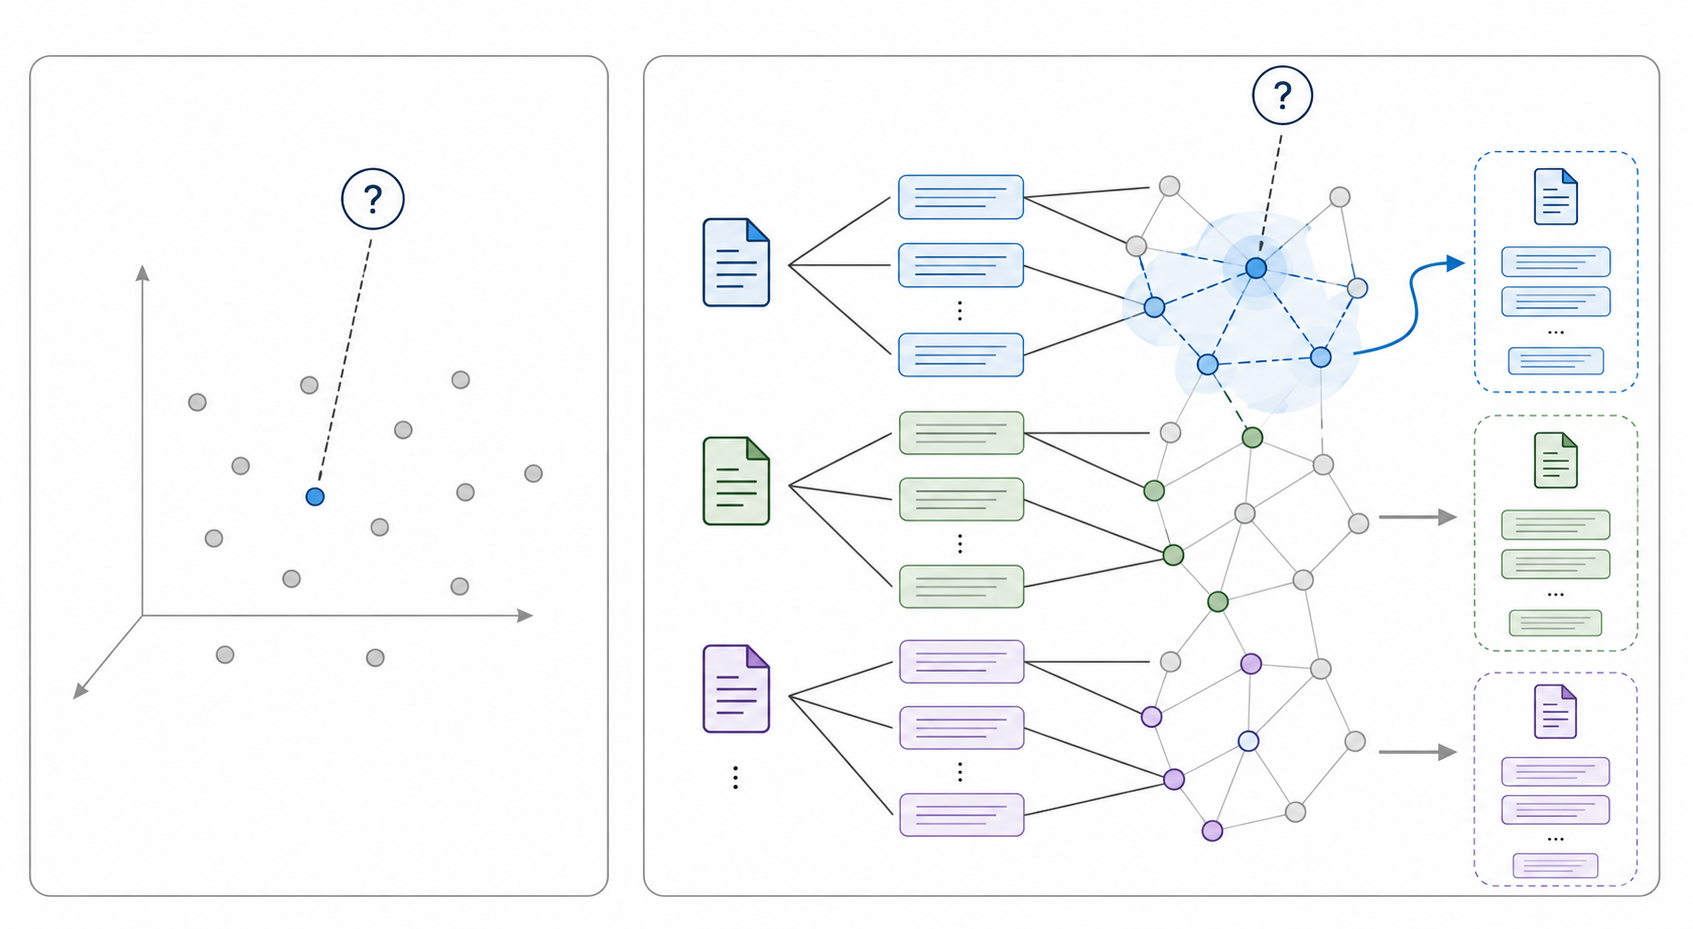
\includegraphics[width=1\textwidth]{_figures/rag_vs_graphrag.png}
    \caption{Confronto concettuale tra un sistema vettoriale ed un sistema ibrido a grafo.}
    \label{fig:rag_vs_graphrag}
\end{figure}

% ─────────────────────────────────────────────────────────────────────────────
\section{Tecnologie Utilizzate}

L'impostazione tecnologica del sistema è stata scelta per garantire un'esecuzione quando più indipendente possibile da servizi esterni, massimizzando performance in termini di latenza e garantendo una sicurezza nella gestione dei dati, i quali non lasciano mai la macchina locale. Di seguito vendono descritte le tecnologie principali utilizzate per lo sviluppo del sistema, con un focus sulle motivazioni che hanno guidato la scelta di ciascuna di esse.

\newpage

% ─────────────────────────────────────────────────────────────────────────────
\subsection{Orchestrazione e Linguaggio}

Il componente principale del sistema, che rappresenta l'unità logica dell'agente conversazionale, è sviluppato in \textbf{Python} \cite{python}, sfruttando il framework \textbf{LangGraph} \cite{langgraph}. La scelta di Python è motivata dall'ampio ecosistema di librerie disponibili per il Machine Learning, la gestione di database e la manipolazione di dati strutturati, che ha permesso di ridurre significativamente i tempi di sviluppo e di integrazione tra i diversi componenti del sistema.

LangGraph in particolare è stato scelto per la sua capacità di modellare flussi di lavoro dinamici, che sono risultati essenziali per la gestione di un Conversational AI basato su RAG. In questo modello ogni nodo del grafo rappresenta un'azione che l'agente può eseguire, e gli archi definiscono le transizioni tra un'azione e la successiva. Questa architettura è risultata fondamentale nello sviluppo del sistema, perché ha permesso di gestire due percorsi di esecuzione distinti. Se la domanda dell'utente è una domanda di conversazione generica, questa può essere gestita direttamente dall'LLM senza accedere al database, eliminando completamente i costi di latenza associati alla ricerca e al recupero dei documenti. Se invece la domanda richiede il recupero di informazioni specifiche, il sistema attiva automaticamente la ricerca dei documenti rilevanti per rispondere alla domanda. Questa flessibilità è stata cruciale per garantire un'esperienza utente fluida e naturale, evitando ritardi inutili per domande che non richiedono accesso alla base di conoscenza.

% ─────────────────────────────────────────────────────────────────────────────
\subsection{Modelli di Intelligenza Artificiale e Hosting Locale}

Il sistema si basa su modelli di intelligenza artificiale eseguiti in locale tramite \textbf{Ollama} \cite{ollama}. Questa scelta è stata dettata sia da considerazioni di sicurezza e privacy, dato che il dominio dei dati è quello medico, sia per abbattere i costi di utilizzo di servizi cloud in termini di costi economici e latenza. I modelli utilizzati per le operazioni di ragionamento ed embedding sono i seguenti:

\begin{itemize}
    \item \textbf{Llama 3.2 (3b)} \cite{dubey2024llama3}: Utilizzato come modello di base per il ragionamento e la generazione del testo. La versione del modello con 3 miliardi di parametri è stata scelta, a confronto con versioni più grandi, per garantire un equilibrio ottimale tra capacità di comprensione e generazione del linguaggio naturale e requisiti computazionali, permettendo un'esecuzione che no comprometta la qualità del servizio senza necessitare di risorse eccessive.

    \item \textbf{Embedding-Gemma} \cite{embedding_gemma_2025}: Utilizzato per la generazione di embedding vettoriali, fondamentali per la ricerca per similarità all'interno del database. Embedding-Gemma è stato scelto per la sua capacità di produrre rappresentazioni semantiche di alta qualità, che migliorano significativamente l'accuratezza della ricerca e del recupero dei documenti rilevanti.
\end{itemize}

% ─────────────────────────────────────────────────────────────────────────────
\subsection{Data Management e Interfaccia}

La gestione dei dati per la base di conoscenza è affidata a \textbf{Neo4j} \cite{neo4j}, un DBMS a grafo che si adatta perfettamente alla rappresentazione strutturata dei documenti utilizzati in questo progetto. Neo4j permette di modellare i documenti come nodi e le relazioni tra essi e le loro porzioni di testo come archi, facilitando la navigazione e il recupero di informazioni. Inoltre, Neo4j supporta nativamente la ricerca per similarità vettoriale, il che ha permesso un'integrazione fluida con il modello di embedding, senza dover ricorrere a soluzioni di terze parti per la gestione dei vettori.

L'interfaccia utente è stata realizzata in \textbf{Unreal Engine} \cite{ue} attraverso il plugin \textbf{FANTASIA} \cite{fantasia1, fantasia2}. FANTASIA è un plugin che consente la creazione facilitata di agenti virtuali intelligenti, fornendo un'integrazione nativa con modelli di intelligenza artificiale e strumenti di orchestrazione come LangGraph. L'utilizzo di Unreal Engine ha permesso di creare un ambiente immersivo e interattivo, in cui l'agente virtuale può rispondere alle domande dell'utente in modo naturale, con supporto per la sintesi vocale e il lip sync, migliorando significativamente l'esperienza utente.

% ─────────────────────────────────────────────────────────────────────────────
\section{Architettura Distribuita e Logica di Sharding}

In scenare reali, applicazioni di conversational AI basate su RAG possono dover gestire basi di conoscenza di dimensioni molto maggiori, con milioni di nodi e relazioni. In questi casi, l'accesso a un database remoto può introdurre una latenza significativa, che si somma a quella del modello di intelligenza artificiale e degli altri componenti del sistema, come la sintesi vocale o il lip sync utilizzato per la maggiore immersività dell'agente virtuale, compromettendo la fluidità dell'interazione \cite{latency_eca} e rendendo vano il vantaggio dell'uso di modelli di intelligenza artificiale.

Per affrontare questo problema, il sistema adotta un'architettura ispirata ai principi del \textit{data sharding} e del \textit{caching} applicati ai database distribuiti \cite{kleppmann2017}. Si noti che, nel corso di una conversazione, l'agente tende ad accedere ripetutamente a un sottoinsieme ristretto dei documenti messi a disposizione. Quindi questo sottoinsieme può essere tenuto in memoria locale per minimizzare il passaggio di dati dal database remoto, riducendo così i costi di latenza e migliorando le performance complessive del sistema. Il database locale funge a tutti gli effetti da cache intelligente, che si aggiorna dinamicamente in base alle esigenze della conversazione e alla frequenza di accesso ai documenti.

\newpage

% ─────────────────────────────────────────────────────────────────────────────
\subsection{Modello a Due Livelli: Remote vs Shard}

Il sistema è quindi strutturato su due livelli distinti per la gestione dei dati:

\begin{enumerate}
    \item \textbf{Remote Storage}: Risiede su un server Neo4j dedicato e contiene l'intera base di conoscenza. Nel caso specifico di questo progetto è stato utilizzato il servizio \textit{Neo4j Aura} per ospitare il database in cloud. Il Remote è il database che viene interrogato per la ricerca iniziale o per recuperare documenti che non sono ancora stati sincronizzati nello Shard locale.

    \item \textbf{Local Shard}: Risiede sulla macchina locale e contiene solo un sottoinsieme dei documenti più rilevanti per la conversazione in corso. Lo Shard funge da cache ad alta velocità, che viene popolata dinamicamente con i documenti recuperati dal Remote. Le query successive alla prima, a meno di cache-miss, resituiscono risultati direttamente dallo Shard, riducendo drasticamente la latenza percepita dall'utente.
\end{enumerate}

Questa separazione trasforma il problema del recupero dati in una strategia di \textbf{caching intelligente}. Quando il sistema recupera informazioni dal Remote, queste vengono sincronizzate nello Shard locale, avvicinando così i dati all'utente. Le interrogazioni successive avverranno direttamente sulla memoria locale, riducendo drasticamente la latenza percepita dall'utente. L'implementazione di questa logica necessita di una gestione del contenuto dello Shard, questo per evitare l'appesantimento dello stesso, che porterebbe inevitabilmente ad un degrado delle performance. Per questo motivo, ad ogni accesso al Remote, il sistema aggiorna dei metadati di utilizzo che alimentano la politica di eviction, garantendo che lo Shard rimanga snello ed efficiente anche nel corso di sessioni prolungate.

\begin{figure}[htbp]
    \centering
    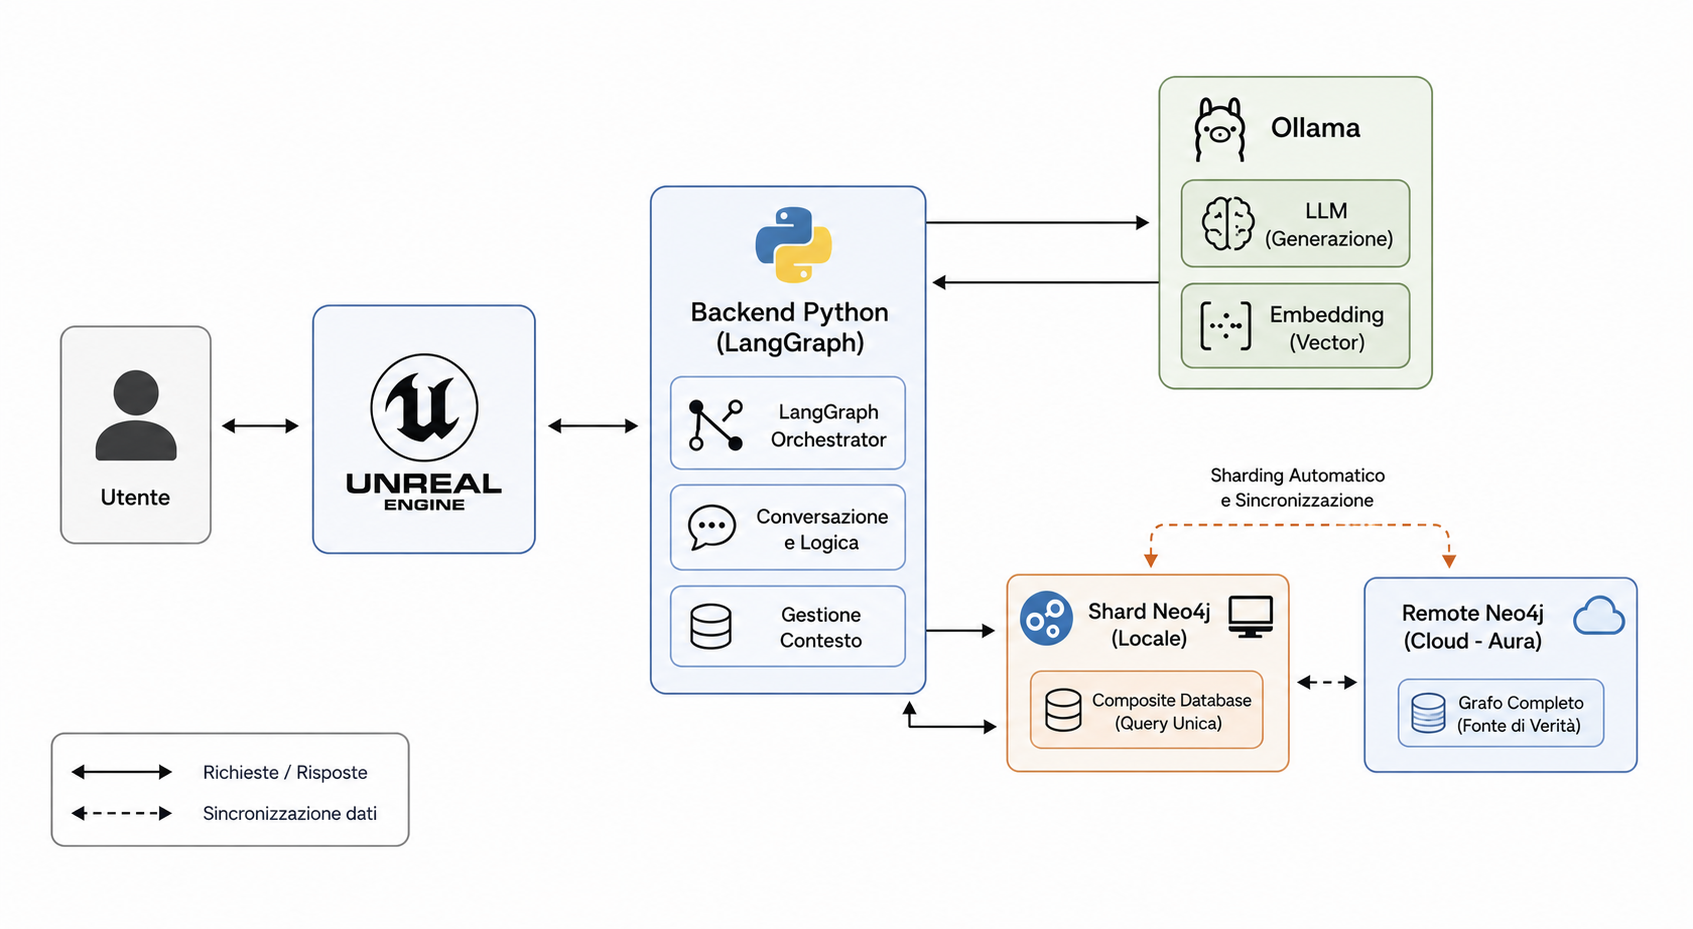
\includegraphics[width=1\textwidth]{_figures/system_architecture.png}
    \caption{Architettura ad alto livello del sistema distribuito.}
    \label{fig:architettura}
\end{figure}

\newpage

% ─────────────────────────────────────────────────────────────────────────────
\section{Ottimizzazione delle Query e Execution Plan Cache}

Un'ulteriore ottimizzazione è stata implementata a livello di query Cypher, per massimizzare le performance del database Neo4j. In un sistema RAG distribuito, la latenza delle query al database è un fattore critico che può influenzare significativamente l'esperienza utente. Per questo motivo, è stato adottato un approccio sistematico all'ottimizzazione delle query, con particolare attenzione alla gestione dell'Execution Plan Cache di Neo4j.

La soluzione è stata quella di parametrizzare le query Cypher, in modo da massimizzare il riutilizzo dei piani di esecuzione. In questo modo, quando una query viene eseguita per la prima volta, Neo4j compila un piano di esecuzione ottimizzato per quella specifica query. Essendo che il sistema è stato strutturato per eseguire tutte le operazioni di sincronizzazione e manutenzione dello Shard locale all'interno della stessa query Cypher, è possibile garantire che lo stesso piano di esecuzione venga riutilizzato costantemente durante la conversazione, riducendo così i tempi di esecuzione delle query successive.

Il beneficio di questa ottimizzazione è doppio, in quanto non solo riduce la latenza delle query al database, ma contribuisce anche a stabilizzare le performance del sistema, evitando picchi di latenza dovuti alla compilazione di nuovi piani di esecuzione per ogni query. Questo è particolarmente importante in un contesto di Conversational AI, dove la reattività del sistema è fondamentale per garantire un'esperienza utente fluida e naturale.

% ─────────────────────────────────────────────────────────────────────────────

\section{Workflow del Sistema}

Il workflow completo del sistema, che integra tutte le componenti descritte nei paragrafi precedenti, può essere sintetizzato nei seguenti passaggi:

\begin{enumerate}
    \item \textbf{Input e Trascrizione}: L'audio dell'utente viene catturato dall'agente virtuale in Unreal Engine e trascritto in testo tramite il modulo \textbf{Whisper ASR} \cite{whisper}, fornito da FANTASIA. La trascrizione viene quindi inviata al server LangGraph.

    \item \textbf{Decisione contestuale}: Il server LangGraph analizza il messaggio dell'utente e determina tramite LLM se si tratta di una domanda di conversazione generica o di una domanda che richiede il recupero di informazioni specifiche. Se è una domanda generica, viene inviata direttamente al modello Llama 3.2 per la generazione della risposta, bypassando completamente il database. Se invece è una domanda che richiede il recupero di informazioni, si attiva la logica di sharding descritta nei passaggi successivi.

    \item \textbf{Ricerca e Sincronizzazione}: Il sistema genera l'embedding del messaggio dell'utente e lo utilizza per eseguire una ricerca per similarità all'interno del Remote Storage. I paragrafi dei documenti più rilevanti vengono recuperati e sincronizzati nello Shard locale insieme ad un contesto di $\pm 2$ paragrafi.

          \newpage

    \item \textbf{Manutenzione (Eviction)}: Ad ogni sincronizzazione, i metadati di utilizzo dei documenti nello Shard vengono aggiornati. Se lo Shard supera una soglia predefinita di capacità, viene attivata la politica di eviction basata su LFU (Least Frequently Used), che rimuove i documenti meno utilizzati per fare spazio a quelli più rilevanti per la conversazione in corso.

    \item \textbf{Generazione e Risposta}: Il modello Llama 3.2 genera una risposta basata sui documenti presenti nello Shard locale, che viene poi restituita a Unreal Engine, il quale tramite il modulo di sintesi vocale \textbf{ElevenLabs} \cite{elevenlabs} genera l'audio risultante che sarà riprodotto dall'agente virtuale.
\end{enumerate}

\begin{figure}[htbp]
    \centering
    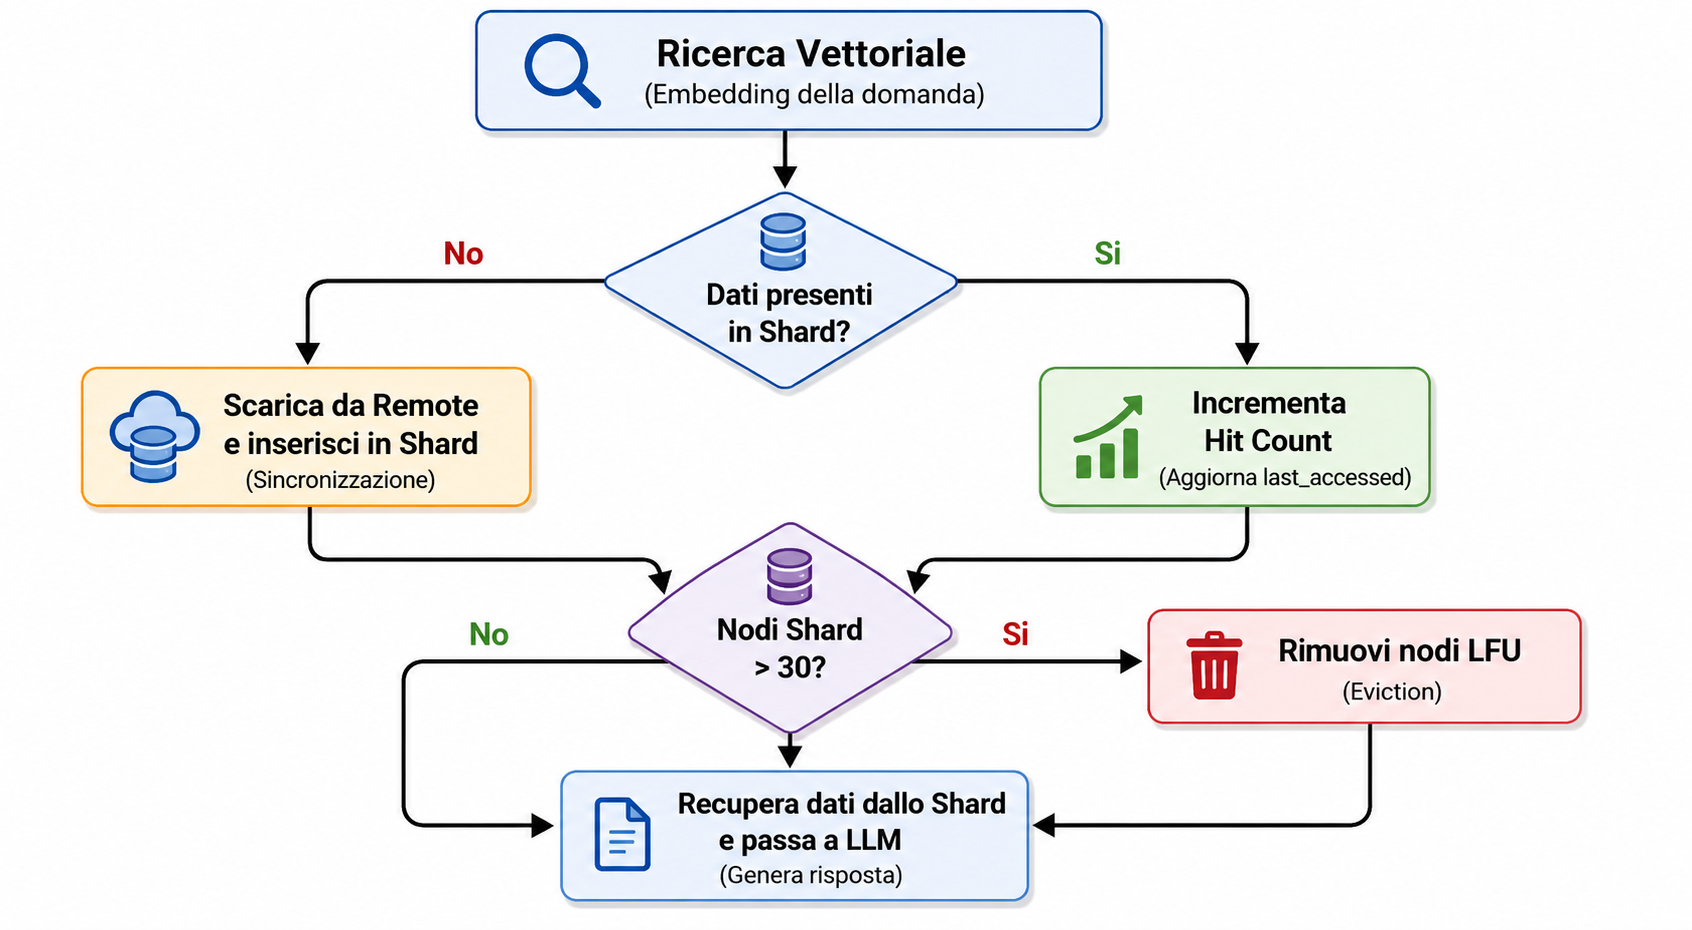
\includegraphics[width=1\textwidth]{_figures/sharding_flowchart.png}
    \caption{Diagramma di flusso della logica di sincronizzazione e manutenzione dello Shard locale.}
    \label{fig:flowchart}
\end{figure}

\begin{figure}[htbp]
    \centering
    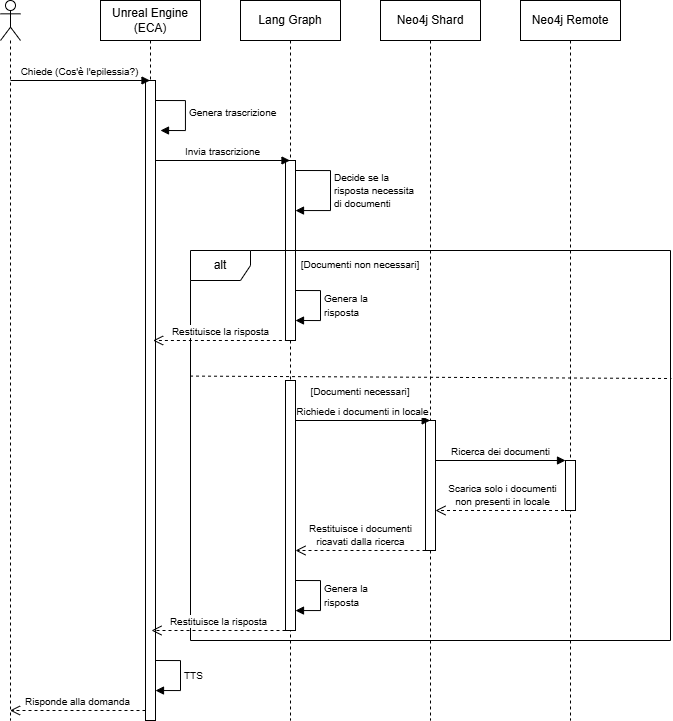
\includegraphics[width=1\textwidth]{_figures/sequence_diagram.png}
    \caption{Sequence diagram dell'interazione completa.}
    \label{fig:sequence}
\end{figure}

\newpage\pagestyle{main}

\chapter{Gestione della Conoscenza e Memoria a Grafo}\label{chap:second}

\inlineminitoc

% ─────────────────────────────────────────────────────────────────────────────
\section{Limiti dei database vettoriali vs. database a grafo}

La maggior parte dei sistemi di Retrieval-Augmented Generation (RAG) \cite{rag_original} attualmente in uso si basano su database vettoriali per memorizzare e recuperare i documenti indicizzati. Questi database sono progettati per eseguire ricerche di similarità su rappresentazioni vettoriali ad alta dimensionalità, e sono estremamente efficienti nel recuperare frammenti di testo che sono semanticamente vicini alla query dell'utente. Tuttavia, questa efficienza viene ottenuta a costo di una perdita significativa di struttura e contesto.

In un contesto dove la natura dei dati è strutturata e gerarchica, la frammentazione dei dati in chunk indipendenti, porta inevitabilmente alla perdita di coerenza e alla difficoltà di ricostruire il contesto originale. Lo scopo di questo lavoro è proprio quello di risolvere questa limitazione fondamentale, integrando un database a grafo che non solo memorizza i documenti indicizzati, ma anche le relazioni strutturali tra di essi, permettendo così di preservare e sfruttare il contesto in modo molto più efficace durante il processo di recupero delle informazioni.

% ─────────────────────────────────────────────────────────────────────────────
\subsection{Frammentazione e perdita di coerenza}

Il limite prinicipale riguarda la perdita di contesto causata dalla frammentazione dei documenti in chunk indipendenti. In un database vettoriale, ogni chunk viene trattato come un'entità isolata, e la ricerca restituisce solo i chunk che presentano la massima similarità con la query. Quindi risulta quasi impossibile recuperare chunk adiacenti che potrebbero essere essenziali per la corretta generazione della risposta.

Una conseguenza pratica di questa frammentazione è che l'LLM potrebbe ricevere solo una porzione del testo che contiene l'informazione chiave, ma senza il contesto necessario per interpretarla correttamente. Ad esempio, un paragrafo che descrive un protocollo di trattamento medico potrebbe essere restituito come risultato della ricerca, ma senza i paragrafi adiacenti che definiscono la condizione clinica o le controindicazioni, l'LLM potrebbe generare una risposta imprecisa o addirittura pericolosa.

Un secondo problema più sottile è legato alla dipendenza semantica tra i chunk. Il sistema potrebbe restituire un chunk che fa uso di termini tecnici o di abbreviazioni che sono definiti solo in un chunk adiacente, e senza quel chunk l'LLM potrebbe non essere in grado di comprendere il significato del testo restituito. In questo senso, la frammentazione non solo riduce la quantità di informazione disponibile, ma anche la qualità dell'informazione stessa, poiché il contesto è spesso essenziale per interpretare correttamente i dati.

% ─────────────────────────────────────────────────────────────────────────────
\subsection{Relazioni Esplicite vs. Implicite}

In un database vettoriale, le relazioni tra i chunk di testo sono solo implicitamente codificate nella vicinanza dei loro embedding. Non esiste una rappresentazione esplicita delle relazioni strutturali o semantiche tra i diversi pezzi di informazione, e il sistema deve affidarsi alla similarità dei vettori per inferire queste relazioni. Questo approccio è intrinsecamente approssimativo e può portare a risultati incoerenti, soprattutto quando la query dell'utente è formulata in modo da richiedere una comprensione più profonda del contesto o delle relazioni tra i concetti.

In un database a grafo, invece, le relazioni sono esplicitamente rappresentate come archi tra i nodi. Questo significa che possiamo definire relazioni specifiche che codificano in modo deterministico le connessioni tra i diversi elementi della Knowledge Base. Questa rappresentazione esplicita consente al sistema di navigare lungo queste relazioni in modo preciso e predicibile, superando la pura approssimazione statistica degli embedding e permettendo di recuperare informazioni correlate in modo più efficace.

\begin{figure}[H]
    \centering
    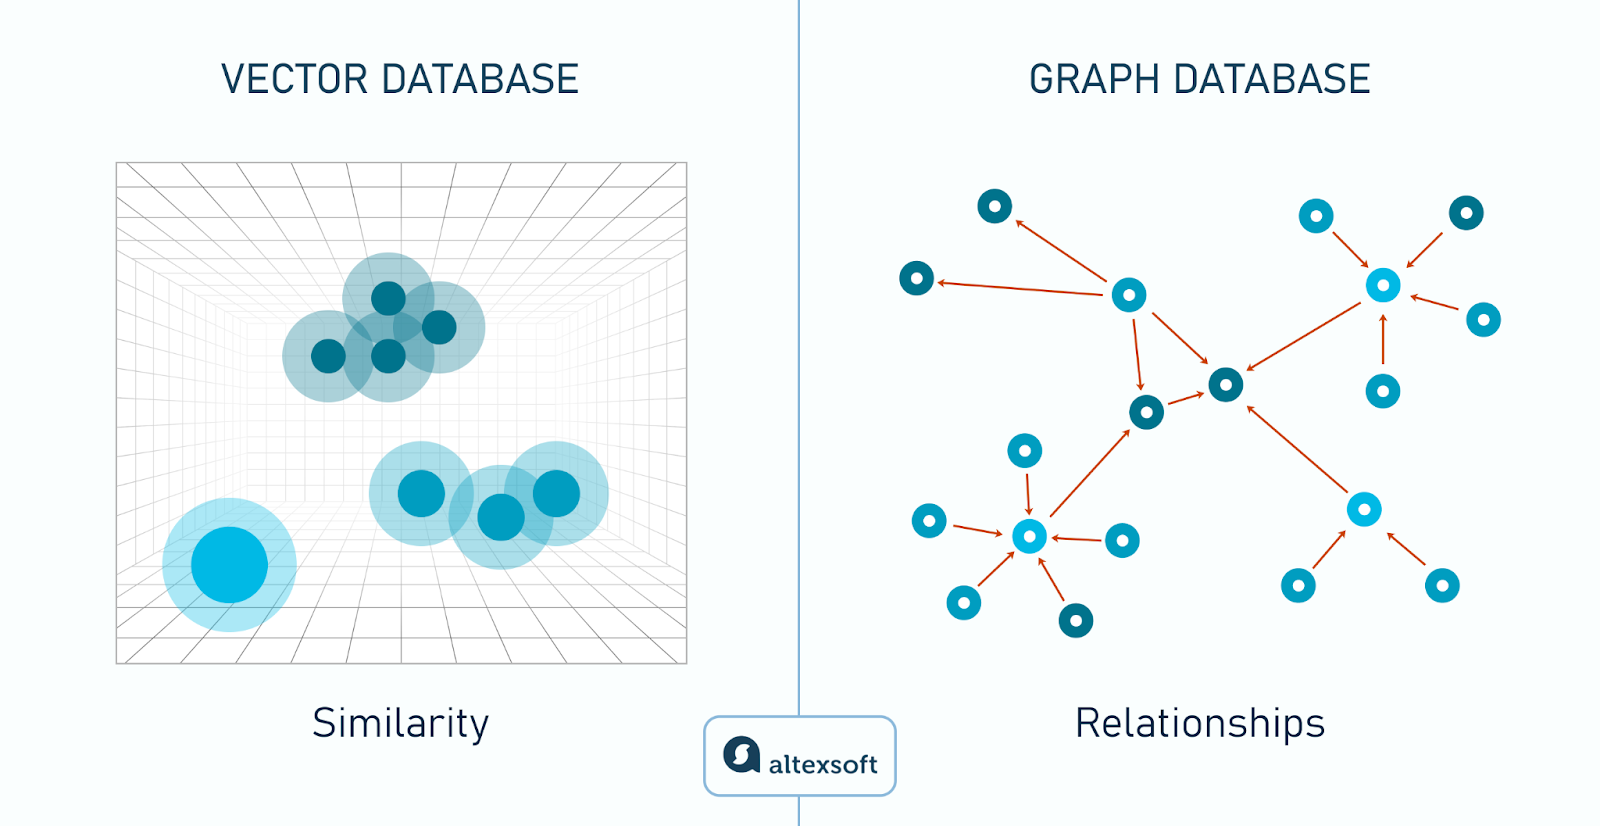
\includegraphics[width=1\textwidth]{_figures/vector_vs_graph_structure.png}
    \caption{Differenza tra memorizzazione lineare e strutturata. Fonte: \url{https://www.altexsoft.com/blog/vector-database/}}
    \label{fig:structure_comp}
\end{figure}

% ─────────────────────────────────────────────────────────────────────────────
\section{Modellazione del Grafo della Conoscenza}

Per questo progetto, è stata utilizzata una struttra dei dati che ha permesso di rappresentare in modo efficace sia il testo dei documenti indicizzati sia le relazioni tra di essi. Il documento non è rappresentato come una stringa piatta, ma come un'entità strutturata con una gerarchia interna precisa. Per ogni documento sono presenti anche molteplici rappresentazioni della stessa informazione, le queli vengono utilizzate per massimizzare la qualità del recupero.

Lo schema del grafo è stato progettato per essere flessibile e scalabile, in modo da poter essere facilmente esteso in futuro con nuovi tipi di nodi o relazioni se necessario. La struttura attuale è stata definita sulla base delle esigenze specifiche del dominio medico, ma i principi di modellazione adottati sono generali e possono essere applicati a qualsiasi dominio in cui la conservazione del contesto e delle relazioni tra le informazioni sia cruciale.

% ─────────────────────────────────────────────────────────────────────────────
\subsection{Schema dei Nodi e delle Relazioni}

Il modello implementato prevede i seguenti tipi di nodo e di relazione:

\begin{itemize}
    \item \textbf{Nodo \texttt{Document}}: Rappresenta l'origine dell'informazione, ovvero il documento sorgente da cui è stato estratto il contenuto. Memorizza il titolo del documento e funge da radice della gerarchia per tutti i paragrafi che lo compongono.

    \item \textbf{Nodo \texttt{Paragraph}}: È l'unità atomica di informazione nel grafo. Contiene il testo integrale del paragrafo, la sua posizione ordinale all'interno del documento \\ (\texttt{document\_position}) e, una volta sincronizzato nello Shard locale, i metadati di utilizzo \texttt{hit\_count} e \texttt{last\_accessed}. La proprietà \texttt{document\_position} è il parametro chiave per il context windowing.

    \item \textbf{Nodo \texttt{Question}}: Rappresenta una domanda tipo che l'utente potrebbe porre per ottenere l'informazione contenuta nel paragrafo collegato. Queste sono state generate automaticamente durante la fase di indicizzazione tramite una chiamata all'LLM. Aggiungere questi nodi consente di migliorare il recuper dei dati, poiché l'utente tenderà a fare domande che saranno di conseguenza più simili alle domande generate, aumentando la probabilità di ottenere un punteggio di similarità elevato durante la ricerca vettoriale.

    \item \textbf{Nodo \texttt{Statement}}: Rappresenta un'affermazione chiave estratta sinteticamente dal paragrafo, anch'essa generata automaticamente dall'LLM durante l'indicizzazione. Mentre le domande rappresentano interrogativi che possono essere associati al paragrafo, le affermazioni rappresentano sintesi assertive del contenuto, e possono essere utili per recuperare informazioni in modo più efficace nel caso di messaggi dell'utente formulati in modo affermativo.

    \item \textbf{Nodo \texttt{Embedding}}: Rappresenta la vera e propria codifica vettoriale di un paragrafo, di una domanda o di un'affermazione. Questi nodi contengono un array di numeri che rappresenta la loro posizione nello spazio vettoriale. La presenza di questi nodi è fondamentale per la ricerca per similarità.

    \item \textbf{Relazione \texttt{HAS\_PARAGRAPH}}: Collega un nodo \texttt{Document} ai suoi nodi \texttt{Paragraph}, codificando la struttura gerarchica del documento. Questa relazione è fondamentale per il context windowing. Data una lista di paragrafi recuperati, il sistema risale al documento genitore e da lì recupera tutti i paragrafi con posizione compresa nell'intervallo di interesse.

    \item \textbf{Relazione \texttt{HAS\_QUESTION}}: Collega un nodo\texttt{Paragraph} alle sue domande associate, permettendo al sistema di navigare bidirezionalmente tra un paragrafo e le interrogazioni che rappresentano il suo contenuto.

    \item \textbf{Relazione \texttt{HAS\_STATEMENT}}: Collega un nodo \texttt{Paragraph} alle sue affermazioni chiave, con lo stesso scopo di \texttt{HAS\_QUESTION} ma per le rappresentazioni di tipo assertivo.

    \item \textbf{Relazione \texttt{HAS\_EMBEDDING}}: Collega un nodo testuale (\texttt{Paragraph}, \texttt{Question} o \texttt{Statement}) al suo embedding vettoriale corrispondente, completando il collegamento tra la rappresentazione simbolica e quella subsimbolica dell'informazione.
\end{itemize}

\begin{figure}[!htbp]
    \centering
    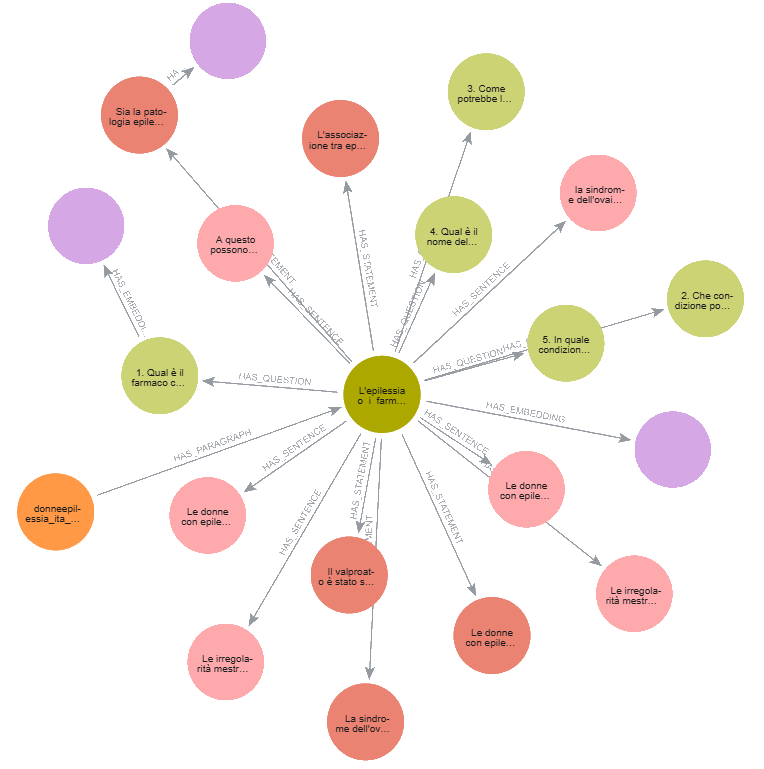
\includegraphics[width=0.95\textwidth]{_figures/graph_metamodel.png}
    \caption{Metamodello del database: nodi \texttt{Document}, \texttt{Paragraph},
        \texttt{Question}, \texttt{Statement} ed \texttt{Embedding} con le rispettive
        relazioni. Il grafo raffigurato è estratto da una porzione della Knowledge Base
        medica relativa al tema dell'epilessia, e mostra come un singolo nodo
        \texttt{Paragraph} sia connesso a più domande, affermazioni ed embedding.}
    \label{fig:metamodel}
\end{figure}

\newpage

% ─────────────────────────────────────────────────────────────────────────────
\section{Rappresentazione Vettoriale e Indicizzazione}

Come spiegato nella sezione precedente, ogni nodo testuale del grafo è collegato a un nodo \texttt{Embedding} che contiene la sua rappresentazione vettoriale. Questa rappresentazione è fondamentale per il processo di recupero, poiché consente di eseguire ricerche per similarità tra la query dell'utente e i contenuti della Knowledge Base. La fase di indicizzazione dei documenti prevede quindi non solo l'estrazione del testo e la creazione dei nodi testuali, ma anche la generazione degli embedding corrispondenti tramite un modello di embedding locale.

% ─────────────────────────────────────────────────────────────────────────────
\subsection{Processo di Embedding con Ollama}

Quando l'utente pone una domanda che necessita di documenti per essere risolta, il sistema deve prima trasformare il testo della query nello stesso spazio vettoriale in cui sono stati proiettati i contenuti della Knowledge Base, in modo da poter calcolare la similarità. Il processo viene eseguito in due operazioni principali:

\begin{enumerate}
    \item Il testo della query viene trascritto da Whisper e inviato al modello di embedding \textit{Embedding-Gemma} \cite{embedding_gemma_2025} in esecuzione locale tramite l'ecosistema \textbf{Ollama} \cite{ollama}. Il modello genera il vettore corrispondente in tempo reale, senza che la query lasci l'infrastruttura locale.

    \item Il vettore della query viene inviato a Neo4j, che esegue una ricerca sul Vector Index configurato sugli embedding della Knowledge Base. Il risultato è una lista ordinata di nodi \texttt{Embedding} con il relativo punteggio di similarità coseno, da cui il sistema risale ai nodi testuali tramite la relazione dedicata.

\end{enumerate}

È importante sottolineare che sia la generazione degli embedding presenti nella Knowledge Base sia la generazione dell'embedding della query avvengono utilizzando lo stesso modello, questo per garantire la massima coerenza nello spazio vettoriale e quindi la massima efficacia nella ricerca per similarità. L'utilizzo di un modello di embedding locale, inoltre, consente di mantenere il controllo completo sui dati e di evitare problemi di latenza o di privacy associati all'invio di query a servizi esterni.

% ─────────────────────────────────────────────────────────────────────────────
\subsection{Vector Index e Similarity Search}

All'interno di Neo4j è stato configurato un \textbf{Vector Index} \cite{neo4j_vector_search} che utilizza l'algoritmo di \textbf{similarità del coseno}. La similarità del coseno misura il coseno dell'angolo tra due vettori nello spazio ad alta dimensionalità, risultando indipendente dalla loro norma e quindi particolarmente adatta a confrontare rappresentazioni testuali, dove la direzione del vettore codifica il significato semantico. Il calcolo della similarità del coseno è espresso dalla seguente formula:

\begin{equation}
    \cos(\theta) = \frac{\mathbf{A} \cdot \mathbf{B}}{\|\mathbf{A}\| \|\mathbf{B}\|}
    \label{eq:cosine}
\end{equation}

dove $\mathbf{A}$ è il vettore del messaggio utilizzato nella query e $\mathbf{B}$ è il vettore del testo ricercato nel database. Un valore di $\cos(\theta)$ pari a 1 indica vettori identici (massima similarità), mentre un valore pari a 0 indica vettori ortogonali (nessuna similarità semantica).

Il sistema esegue una ricerca ordinata per similarità, restituendo i nodi \texttt{Embedding} con i punteggi più alti. Tuttavia, non tutti i risultati vengono considerati validi per la fase di recupero. Viene applicata una soglia di confidenza (80\%) che filtra i risultati in base al loro punteggio di similarità. Questo viene fatto per garantire che solo i risultati più pertinenti vengano utilizzati per la generazione della risposta, evitando che l'LLM si basi su contesti debolmente correlati alla domanda dell'utente, che potrebbero portare a risposte imprecise o fuorvianti. La scelta di questa soglia è stata determinata empiricamente durante la fase di sviluppo, bilanciando la necessità di recuperare informazioni rilevanti con il rischio di includere dati non pertinenti.

% ─────────────────────────────────────────────────────────────────────────────
\section{Strategie di Recupero e Navigazione del Contesto}
\label{sec:context_windowing}

Una volta indivituato il paragrafo ancora tramite la ricerca vettoriale, il sistema non si limita a restituire solo quel singolo paragrafo all'LLM, ma implementa una strategia di \textbf{context windowing dinamico} che consente di recuperare automaticamente i paragrafi adiacenti, creando così un contesto più ampio e coerente per la generazione della risposta.

% ─────────────────────────────────────────────────────────────────────────────
\subsection{Context Windowing Dinamico}

Invece di restituire solo il paragrafo ancora, il sistema risale al nodo \texttt{Document} genitore e recupera tutti i paragrafi con posizione compresa nell'intervallo di $\pm 2$ posizioni rispetto al paragrafo ancora. In questo modo viene creata una finestra di contesto che include fino a cinque paragrafi consecutivi. Questo non solo aumenta l'accuratezza della risposta fornendo più contesto, ma nella formula dello shard utilizzato come cache, consente di predirre domande future che potrebbero essere correlate a quei paragrafi adiacenti, aumentando così la probabilità di cache hit nelle query successive.

La finestra di $\pm 2$ posizioni è stata scelta come compromesso tra la necessità di fornire un contesto sufficiente e il rischio di includere informazioni troppo distanti che potrebbero non essere rilevanti per la domanda dell'utente. Questa strategia consente di mantenere un equilibrio tra la coerenza del contesto e la pertinenza delle informazioni fornite all'LLM, migliorando significativamente la qualità delle risposte generate, ed evitando di incrementare inutilmente la dimensione dello shard locale.

\begin{figure}[H]
    \centering
    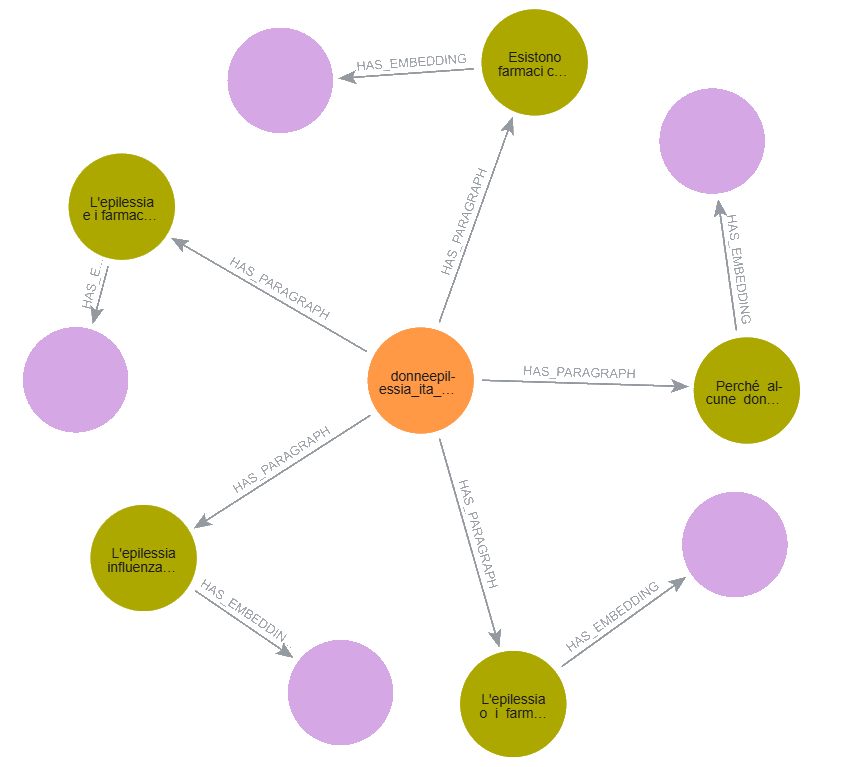
\includegraphics[width=1\textwidth]{_figures/context_expansion_logic.png}
    \caption{Visualizzazione del documento con la finestra di contesto.}
    \label{fig:context_expansion}
\end{figure}

% ─────────────────────────────────────────────────────────────────────────────
\subsection{Vantaggi della navigazione sequenziale}

Questa strategia offre numerosi vantaggi rispetto a un approccio che restituisce solo il paragrafo ancora. Innanzitutto, consente di preservare la coerenza del testo, poiché i paragrafi adiacenti spesso contengono informazioni che si riferiscono direttamente al paragrafo ancora, e che sono essenziali per una corretta interpretazione del contenuto. In secondo luogo, migliora la capacità dell'LLM di generare risposte più accurate e complete, poiché ha accesso ad un contesto più ricco e dettagliato.

I benefici di questo approccio sono particolarmente evidenti in documenti tecnici o medici, dove la comprensione di un concetto dipende strettamente dalle definizioni fornite nelle righe precedenti. Un paragrafo che descrive il protocollo di somministrazione di un farmaco antiepilettco, per esempio, acquisisce significato completo solo se l'LLM ha accesso anche al paragrafo precedente che definisce la condizione clinica per cui quel farmaco è indicato. Con il context windowing, questa informazione è sempre disponibile, indipendentemente da quale paragrafo sia stato il migliore risultato della ricerca vettoriale.

Un ulteriore vantaggio riguarda la robustezza rispetto a domande formulate in modo parziale o indiretto. Anche se il paragrafo ancora non contiene tutte le informazioni necessarie per rispondere, i paragrafi adiacenti spesso le completano, riducendo la probabilità che l'LLM si trovi costretto a dedurre informazioni non presenti nel contesto.

% ─────────────────────────────────────────────────────────────────────────────
\section{Implementazione dello Sharding e Sincronizzazione}

Un aspetto cruciale di questa tesi è il passaggio dei dati dal database remoto allo Shard locale. Questo processo non è una semplice copia dei dati: è una strategia dinamica che tiene traccia dell'utilizzo di ogni nodo nel tempo, e che usa queste informazioni sia per decidere quali dati mantenere in cache sia per garantire che le interrogazioni successive possano essere soddisfatte localmente il più spesso possibile.

% ─────────────────────────────────────────────────────────────────────────────
\subsection{Logica di Hit-Rate}

Ogni volta che un nodo viene recuperato dal database remoto, il sistema non si limita a restituirlo all'LLM come risultato della ricerca, ma lo proietta anche nello Shard locale tramite un'operazione di upsert. Il termine upsert indica una scrittura condizionale. Se il nodo non è ancora presente nello Shard, viene creato con \texttt{hit\_count = 1}, se invece è già presente, vengono aggiornati solo i suoi metadati di utilizzo.

Nello specifico, il sistema incrementa la proprietà \texttt{hit\_count} di una unità e aggiorna la proprietà \texttt{last\_accessed} con il timestamp corrente. Questa proprietà, in combinazione con il timestamp, è fondamentale per la politica di gestione della memoria. I nodi con un alto \texttt{hit\_count} e un timestamp recente sono considerati \textbf{``conoscenza calda''}, ovvero informazioni che l'utente ha consultato frequentemente di recente e che ha quindi alta probabilità di consultare nuovamente nel corso della stessa sessione. Questi nodi hanno la massima priorità di permanenza nello Shard e saranno gli ultimi ad essere rimossi quando si attiva la politica di eviction.

Questa logica di tracciamento dell'utilizzo consente al sistema di adattarsi dinamicamente alle esigenze dell'utente, mantenendo nello shard le informazioni più rilevanti e frequenti, e rimuovendo quelle che sono state consultate meno spesso o che non sono state consultate da molto tempo. In questo modo, lo Shard locale diventa una rappresentazione dinamica e adattiva della conoscenza più pertinente per l'utente, migliorando significativamente la latenza delle risposte e l'efficacia del recupero delle informazioni durante la sessione conversazionale.

\newpage

% ─────────────────────────────────────────────────────────────────────────────
\subsection{Algoritmo di Eviction LFU (Least Frequently Used)}

Per garantire che lo Shard locale non cresca indefinitamente e non saturi la memoria del dispositivo su cui è in esecuzione l'agente, è stata implementata una soglia massima di 30 nodi \texttt{PARAGRAPH}. Questa soglia rappresenta il limite superiore della dimensione della cache locale, e viene monitorata costantemente durante l'esecuzione dell'agente.

Quando il numero di nodi \texttt{PARAGRAPH} nello Shard supera la soglia di 30, viene attivata automaticamente una procedura di pulizia che ha lo scopo di riportare il numero di nodi alla soglia, rimuovendo il numero minimo di nodi necessario. La procedura di pulizia si basa su un algoritmo di eviction denominato \textbf{Least Frequently Used (LFU)}, che privilegia la rimozione dei nodi acceduti con minore frequenza.

Questa politica è stata scelta perché si adatta meglio alla natura delle sessioni conversazionali mediche, dove un paziente che chiede più volte informazioni sullo stesso argomento indica un interesse consolidato per quel topic, e i dati correlati devono rimanere in cache anche se non sono stati acceduti nell'ultima query. Al contrario, nodi che sono stati consultati solo una volta o che non sono stati consultati da molto tempo hanno una probabilità molto più bassa di essere rilevanti per le domande future, e quindi vengono rimossi per fare spazio a nuove informazioni più pertinenti.

\newpage\pagestyle{main}

\chapter{Sviluppo del Sistema: Distribuzione e Sincronizzazione}\label{chap:third}

\inlineminitoc

% ─────────────────────────────────────────────────────────────────────────────
\section{Logica dello Sharding: Gestione dinamica dei dati}

In un ecosistema di Intelligenza Artificiale Conversazionale, la velocità di risposta
è un fattore critico per l'accettazione da parte dell'utente \cite{latency_eca}.
La percezione di naturalezza in un dialogo con un agente virtuale dipende in misura
significativa dalla latenza: risposte che arrivano dopo più di qualche secondo
interrompono il flusso conversazionale e degradano l'esperienza utente, indipendentemente
dalla qualità del contenuto della risposta stessa. In contesti come quello medico,
dove l'utente può trovarsi in uno stato di preoccupazione o urgenza, questo aspetto
diventa ancora più rilevante.

Il problema fondamentale è un \textbf{trade-off} tra completezza e velocità. Da un
lato, la base di conoscenza deve essere completa e aggiornata, il che richiede di
mantenerla su un server centrale accessibile da qualsiasi istanza del sistema. Dall'altro,
ogni interrogazione a un database remoto introduce una latenza di rete che, sommata
agli altri tempi di elaborazione del sistema, può superare facilmente la soglia di
tollerabilità. Il caricamento dell'intera base di conoscenza in memoria locale
sarebbe la soluzione ideale in termini di velocità, ma è spesso impraticabile: un
database medico realistico può contenere milioni di nodi, e trasferire e mantenere
sincronizzata una copia locale di queste dimensioni richiederebbe risorse computazionali
e di storage non disponibili su hardware consumer.

Per risolvere questo trade-off, il sistema adotta una logica di \textbf{sharding}
basata sulla distinzione tra due livelli di memorizzazione con caratteristiche
complementari:

\begin{itemize}
    \item \textbf{Remote Knowledge Base}: Un repository completo e persistente,
          ospitato su un server centrale, che contiene la totalità delle informazioni
          disponibili. È la fonte di verità del sistema: aggiornata centralmente, sempre
          coerente, ma soggetta a latenza di rete variabile a ogni interrogazione.

    \item \textbf{Local Shard}: Una memoria ad alte prestazioni, situata sullo
          stesso host che esegue il backend Python e i modelli Ollama, che contiene
          solo il sottoinsieme di dati rilevante per la sessione conversazionale corrente.
          Essendo locale, le sue interrogazioni avvengono senza latenza di rete, con
          tempi di risposta paragonabili a quelli di un accesso in memoria.
\end{itemize}

Questa architettura si ispira ai concetti di \textit{Caching} e \textit{Data Sharding}
descritti da Kleppmann \cite{kleppmann2017}, adattandoli però alle necessità specifiche
dei database a grafo, dove la \textbf{vicinanza topologica} tra i nodi è altrettanto
importante della vicinanza temporale degli accessi. Nei database relazionali o
documentali tradizionali, una strategia di caching basata sulle singole righe o
documenti più acceduti è sufficiente. In un database a grafo, invece, è fondamentale
portare in cache non solo il nodo richiesto, ma anche i suoi vicini strutturali —
i paragrafi adiacenti nel documento, il nodo documento genitore — perché è la
navigazione di questi collegamenti, e non il nodo isolato, a fornire il contesto
ricco necessario all'LLM.

\begin{figure}[htbp]
    \centering
    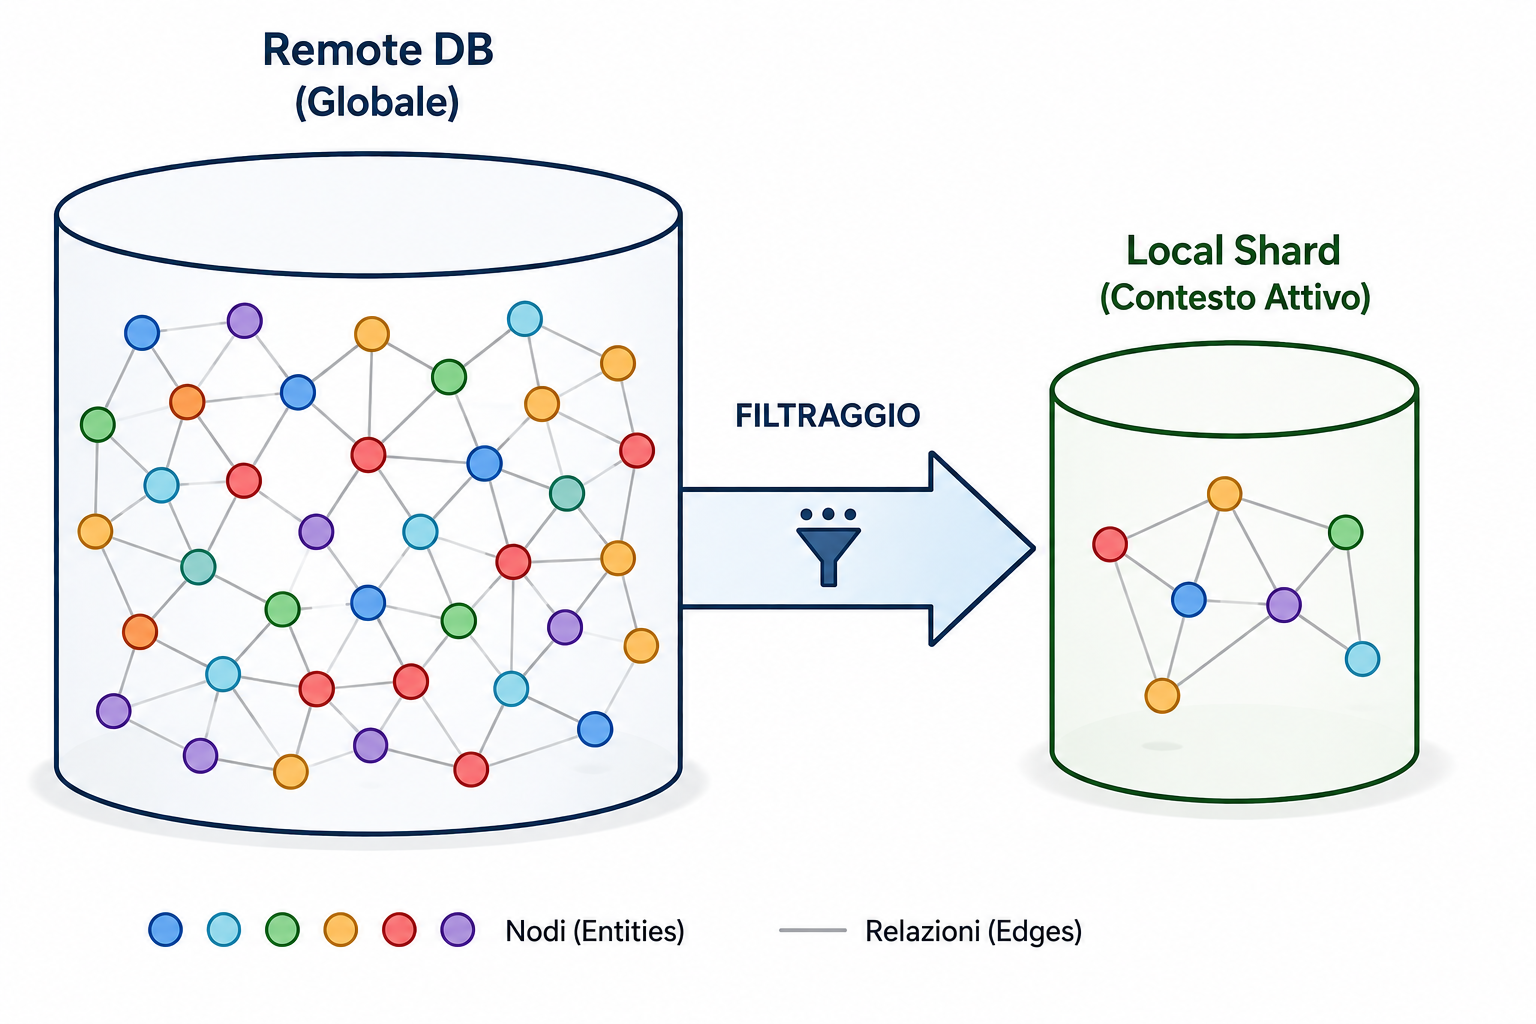
\includegraphics[width=0.8\textwidth]{_figures/sharding_levels.png}
    \caption{Rappresentazione dei due livelli di memorizzazione: Remote DB (Globale)
        e Local Shard (Contesto Attivo). Il filtraggio selettivo garantisce che solo i
        dati ``caldi'' — quelli acceduti frequentemente nella sessione corrente — vengano
        mantenuti nello Shard locale, mentre il Remote rimane la fonte di verità completa.}
    \label{fig:sharding_levels}
\end{figure}

% ─────────────────────────────────────────────────────────────────────────────
\section{Il ciclo di vita della query distribuita}

L'interazione con il sistema non è una semplice operazione di lettura su un singolo
database, ma un \textbf{processo ciclico} coordinato dall'orchestratore Python tramite LangGraph. Ogni volta che l'agente necessita di recuperare informazioni dalla Knowledge Base, viene eseguita una sequenza di operazioni che attraversa entrambi i livelli dell'architettura distribuita: il Remote, per la ricerca vettoriale sull'indice completo, e lo Shard locale, per la sincronizzazione, la manutenzione della cache e il recupero finale del contesto da fornire all'LLM.
Il cuore tecnologico di questo processo è l'integrazione tra la ricerca vettoriale
e la manipolazione del grafo in un'unica transazione atomica, realizzata sfruttando
le funzionalità avanzate di Neo4j per la gestione di database compositi distribuiti.

% ─────────────────────────────────────────────────────────────────────────────
\subsection{L'uso delle Call Subqueries}

Per implementare questa logica complessa in Neo4j mantenendo al contempo l'atomicità
dell'operazione, si è fatto ricorso alle \textbf{Call Subqueries} \cite{neo4j_subqueries}.
Le Call Subqueries permettono di eseguire blocchi di logica Cypher separati all'interno
di una query principale, specificando per ciascuno su quale database del cluster deve
essere eseguito tramite la clausola \texttt{USE}. Questa funzionalità è la chiave
che rende possibile coordinare operazioni su database fisicamente distinti — il Remote
e lo Shard — nell'ambito di un'unica chiamata dal layer applicativo Python.

La scelta di accentrare tutta la logica in un'unica macro-query, anziché distribuirla
su più chiamate separate dal codice Python, è motivata da ragioni sia di prestazioni
sia di correttezza. Dal punto di vista delle prestazioni, ogni chiamata da Python al
database comporta un overhead di serializzazione, trasmissione di rete e
deserializzazione. Ridurre il numero di round-trip significa ridurre proporzionalmente
questo overhead: con la macro-query, Python effettua una sola chiamata e riceve un
solo risultato, indipendentemente dalla complessità delle operazioni eseguite
internamente. Senza questa funzionalità, il sistema dovrebbe scaricare i dati in
Python, elaborarli in memoria e reinviarli al database locale, potenzialmente
raddoppiando i tempi di comunicazione.

Dal punto di vista della correttezza, avere tutta la logica in una singola transazione
garantisce che le operazioni di lettura dal Remote e di scrittura sullo Shard siano
coerenti tra loro: non è possibile che una lettura riesca e la scrittura successiva
fallisca lasciando lo Shard in uno stato parziale, perché entrambe le operazioni
fanno parte della stessa unità di lavoro transazionale. Con le subqueries, lo
spostamento dei dati tra Remote e Shard avviene in modo quasi trasparente per
l'applicazione Python, che vede semplicemente una chiamata con un parametro
(il vettore della query) e un risultato (i paragrafi contestuali da fornire all'LLM).

Un ulteriore vantaggio delle Call Subqueries è la possibilità di implementare
\textbf{logica condizionale} tramite la sintassi \texttt{WHEN...THEN}. Questa funzionalità è
fondamentale per la logica di \textit{upsert}: in base al fatto che un nodo sia
già presente o meno nello Shard, il sistema esegue azioni diverse — creazione ex
novo o semplice aggiornamento dei metadati — senza dover uscire dalla query per
effettuare questo controllo a livello applicativo.

\newpage

% ─────────────────────────────────────────────────────────────────────────────
\section{Implementazione della logica di sincronizzazione}

Di seguito viene analizzata nel dettaglio la macro-query Cypher che governa l'intero
processo di recupero e aggiornamento. La query è strutturata in quattro blocchi
funzionali distinti, ognuno dei quali esegue una fase specifica del ciclo di vita
della query distribuita. La suddivisione in blocchi non è solo una scelta stilistica:
ciascun blocco opera su un contesto di dati diverso e, nel caso dei blocchi che
utilizzano la clausola \texttt{USE}, su un database fisicamente diverso.

% ─────────────────────────────────────────────────────────────────────────────
\subsection{Fase 1: Ricerca Vettoriale e Identificazione}

La prima fase interroga l'indice vettoriale del database remoto per identificare
i paragrafi più pertinenti alla query dell'utente e per espandere il contesto
attorno a ciascuno di essi. Non ci si limita a cercare il singolo nodo più simile:
il sistema recupera i migliori risultati tra tutti i candidati con score sufficiente,
per poi estrarre i metadati necessari alla ricostruzione del contesto locale per
ciascuno di essi.

\begin{lstlisting}[language=Cypher, breaklines=true, caption={Ricerca Vettoriale e Identificazione dei Paragrafi Rilevanti}, label=lst:vector_search]
    // 1. RICERCA SU REMOTE
    CALL () {
        USE composite.remote
        CALL db.index.vector.queryNodes('embeddingIndex', 1000, $embedding)
        YIELD node AS emb, score
        FILTER score >= 0.80
        MATCH (emb)<-[:HAS_EMBEDDING]-(p:PARAGRAPH)
        ORDER BY score DESC LIMIT 10
        WITH collect(p) as topParag
        UNWIND topParag as parag
        MATCH (doc:DOCUMENT)-[:HAS_PARAGRAPH]->(parag)
        WITH DISTINCT doc, parag
        MATCH (doc)-[:HAS_PARAGRAPH]->(candidate:PARAGRAPH)
        WHERE candidate.document_position IN [
            parag.document_position - 2,
            parag.document_position - 1,
            parag.document_position,
            parag.document_position + 1,
            parag.document_position + 2
        ]
        RETURN
            elementId(doc) as rid_doc,
            properties(doc) as props_doc,
            elementId(candidate) as rid_parag,
            properties(candidate) as props_parag
    }
\end{lstlisting}

\vspace{1.5em}

Vale la pena analizzare le scelte implementative di questo blocco con attenzione.
La chiamata \texttt{db.index.vector.queryNodes} riceve tre argomenti: il nome
dell'indice vettoriale (\texttt{'embeddingIndex'}), il numero massimo di candidati
da esaminare, e il vettore della query \texttt{\$embedding} come parametro
parametrizzato. Il \texttt{FILTER score >= 0.80} scarta immediatamente i candidati
con similarità insufficiente, prima di qualsiasi operazione di navigazione sul grafo,
limitando il lavoro delle fasi successive.

La navigazione \texttt{(emb)<-[:HAS\_EMBEDDING]-(p:PARAGRAPH)} risale dall'embedding
al nodo testo corrispondente, sfruttando la struttura ibrida del grafo descritta nel
Capitolo \ref{chap:second}. Dopo aver raccolto e de-duplicato i paragrafi ancora nei top-10 per
similarità, la query risale al documento genitore (\texttt{MATCH (doc:DOCUMENT)-[:HAS\_PARAGRAPH]->(parag)}) e da lì recupera tutti i candidati nella finestra
contestuale di $\pm 2$ posizioni. Il risultato di questa fase è un insieme di righe,
ciascuna delle quali descrive un paragrafo candidato (con tutte le sue proprietà) e
il documento a cui appartiene, pronto per essere processato dalla fase successiva.

% ─────────────────────────────────────────────────────────────────────────────
\subsection{Fase 2: Proiezione e Incremento del Hit-Rate}

Una volta identificati i paragrafi rilevanti e i loro vicini contestuali, il sistema
deve ``proiettarli'' nello Shard locale tramite la logica di \textit{upsert}. Questa
fase opera sul database locale (\texttt{USE composite.shard}) e riceve in input i
metadati di ciascun paragrafo candidato prodotti dalla fase precedente.

\begin{lstlisting}[language=Cypher, caption={Logica di Upsert e sincronizzazione dei nodi}, label=lst:upsert]
    // 2. SINCRONIZZAZIONE E AGGIORNAMENTO HIT-RATE SU SHARD
    CALL (rid_doc, props_doc, rid_parag, props_parag) {
        USE composite.shard
        OPTIONAL MATCH (p:PARAGRAPH {remote_id: rid_parag})
        WITH p, (p IS NULL) as isMiss, rid_doc, props_doc, rid_parag,
             props_parag

        WITH p, isMiss, rid_doc, props_doc, rid_parag, props_parag
        CALL (p, isMiss, rid_doc, props_doc, rid_parag, props_parag){
            WHEN isMiss THEN {
                MERGE (d:DOCUMENT {remote_id: rid_doc})
                SET d += props_doc
                MERGE (newP:PARAGRAPH {remote_id: rid_parag})
                SET newP += props_parag,
                    newP.hit_count = 1,
                    newP.last_accessed = datetime()
                MERGE (d)-[:HAS_PARAGRAPH]->(newP)
                RETURN rid_parag as sync_id
            }
            ELSE {
                SET p.hit_count = p.hit_count + 1,
                    p.last_accessed = datetime()
                RETURN rid_parag as sync_id
            }
        }
        RETURN sync_id
    }
\end{lstlisting}

\vspace{1.5em}

La struttura di questo blocco merita un'analisi approfondita. L'\texttt{OPTIONAL MATCH}
iniziale è la chiave del meccanismo di \textit{upsert}: tenta di trovare nello Shard
un nodo \texttt{PARAGRAPH} con il \texttt{remote\_id} corrispondente all'ID del
paragrafo sul Remote, e se non lo trova restituisce \texttt{NULL} anziché produrre
un errore. Il flag booleano \texttt{isMiss} viene quindi calcolato come
\texttt{(p IS NULL)}, distinguendo tra i due casi del ramo condizionale successivo.

Nel ramo \texttt{WHEN isMiss THEN} — il \textit{cache miss} — la query utilizza
\texttt{MERGE} sia per il nodo \texttt{DOCUMENT} sia per il nodo \texttt{PARAGRAPH}.
L'uso di \texttt{MERGE} anziché \texttt{CREATE} è fondamentale: \texttt{MERGE}
crea il nodo solo se non esiste già, e altrimenti non fa nulla, garantendo
l'\textbf{idempotenza} dell'operazione. Questo significa che, anche se la stessa
query venisse eseguita due volte per lo stesso paragrafo a causa di un errore di rete
o di un ritentativo, non verrebbero creati nodi duplicati nello Shard. Le proprietà
del paragrafo vengono copiate dal Remote tramite \texttt{SET newP += props\_parag},
e i metadati di utilizzo vengono inizializzati: \texttt{hit\_count = 1} e
\texttt{last\_accessed = datetime()}.

Nel ramo \texttt{ELSE} — il \textit{cache hit} — il nodo esiste già nello Shard,
e il sistema si limita ad aggiornare i suoi metadati: il contatore viene incrementato
di una unità e il timestamp viene aggiornato al momento corrente. L'istruzione
\texttt{MERGE} è la garanzia che non vengano creati duplicati nello Shard anche
in scenari di concorrenza o di riesecuzione: se il paragrafo è stato già citato
pochi scambi prima nella stessa sessione, viene solo aggiornato il contatore
delle visite, non ricreato da capo.

% ─────────────────────────────────────────────────────────────────────────────
\section{Gestione della Memoria Locale: Politica di Eviction}

Lo Shard locale deve rimanere snello per non degradare le prestazioni delle
interrogazioni locali. Un database a grafo con migliaia di nodi richiede più
tempo per la pianificazione ed esecuzione delle query rispetto a uno con poche
decine di nodi, anche se i nodi in eccesso non sono direttamente rilevanti per
la query in corso. Per questo motivo è stata implementata una politica di
\textbf{Least Frequently Used (LFU)} combinata con un limite fisico di nodi,
che mantiene la dimensione dello Shard costantemente sotto controllo senza
richiedere processi di manutenzione esterni.

% ─────────────────────────────────────────────────────────────────────────────
\subsection{Algoritmo di pulizia automatica}

Il sistema mantiene un massimo di 30 nodi \texttt{PARAGRAPH} nello Shard. La scelta
di questa soglia specifica riflette un compromesso: un valore troppo basso
aumenterebbe la frequenza dei \textit{cache miss} e dei conseguenti accessi al
Remote, mentre un valore troppo alto ridurrebbe il beneficio prestazionale dello
Shard. Con il dataset di test descritto nel Capitolo \ref{chap:fifth} — circa 600 nodi
\texttt{PARAGRAPH} sul Remote — la soglia di 30 nodi rappresenta circa il 5\%
della Knowledge Base, sufficiente a coprire ampiamente il contesto di una sessione
conversazionale focalizzata su un singolo dominio medico.

Quando il numero di nodi \texttt{PARAGRAPH} nello Shard supera la soglia, i nodi
con il minor numero di \textit{hit} e l'accesso più vecchio vengono eliminati.
Crucialmente, questa logica è implementata \textbf{direttamente nella macro-query
    Cypher}, nello stesso blocco che gestisce la sincronizzazione. Questo significa che
la pulizia avviene in modo sincrono, contestualmente all'inserimento di nuovi nodi,
senza la necessità di processi di manutenzione schedulati esternamente che potrebbero
creare race condition o lasciare lo Shard in uno stato temporaneamente sovradimensionato.

\begin{lstlisting}[language=Cypher, caption={Logica di Eviction basata su LFU e recupero finale}, label=lst:eviction]
    // 3. LOGICA DI EVICTION (PULIZIA) - MAX 30 NODI
    WITH DISTINCT 1 as singleton, sync_id as rid_parag
    CALL (singleton) {
        USE composite.shard
        MATCH (p:PARAGRAPH)
        WITH p ORDER BY p.hit_count ASC, p.last_accessed ASC
        WITH collect(p) as allNodes, size(collect(p)) as total

        WITH allNodes, total
        CALL (allNodes, total) {
            WHEN total > 30 THEN {
                UNWIND allNodes[0..(total-30)] as toDelete
                DETACH DELETE toDelete
                RETURN count() as deletedCount
                }
            ELSE {
                RETURN 0 as deletedCount
            }
        }
        RETURN deletedCount
    }

    // 4. RECUPERO FINALE DALLO SHARD
    WITH DISTINCT rid_parag
    CALL (rid_parag) {
        USE composite.shard
        MATCH (doc:DOCUMENT)-[:HAS_PARAGRAPH]->
            (p:PARAGRAPH {remote_id: rid_parag})
        RETURN
            properties(doc) as docData,
            properties(p) as paragData,
            doc.remote_id as docId
    }

    WITH docData, docId, paragData
    ORDER BY docId, paragData.document_position ASC
    WITH docData, docId, collect(paragData) as paragrafi
    RETURN docData, docId, paragrafi
\end{lstlisting}

\newpage

Il terzo blocco merita un'analisi riga per riga. La query recupera tutti i nodi
\texttt{PARAGRAPH} presenti nello Shard e li ordina in modo crescente per
\texttt{hit\_count} e, a parità di \texttt{hit\_count}, per \texttt{last\_accessed}:
i nodi da eliminare per primi sono quindi quelli acceduti meno volte e meno di recente,
in piena coerenza con la politica LFU. La lista ordinata viene raccolta in
\texttt{allNodes} e la sua dimensione in \texttt{total}.

Il ramo condizionale \texttt{WHEN total > 30 THEN} si attiva solo se la soglia è
stata superata. La slice \texttt{allNodes[0..(total-30)]} estrae esattamente il
numero minimo di nodi da rimuovere per tornare alla soglia: se ad esempio lo Shard
contiene 35 nodi, la slice restituirà i primi 5 (i meno rilevanti), lasciando intatti
i 30 più rilevanti. L'operazione \texttt{DETACH DELETE} rimuove ogni nodo candidato
insieme a tutti i suoi archi, garantendo che lo Shard rimanga un grafo strutturalmente
valido senza relazioni orfane.

Il quarto blocco, il \textbf{recupero finale}, esegue la lettura definitiva dei
paragrafi dallo Shard locale — che a questo punto è stato sincronizzato e ripulito —
e li restituisce al backend Python ordinati per documento e posizione. L'ordinamento
\texttt{ORDER BY docId, paragData.document\_position ASC} garantisce che l'LLM
riceva i paragrafi nell'ordine corretto, ricostruendo fedelmente la sequenza
narrativa del documento originale. Il \texttt{collect(paragData)} raggruppa infine
tutti i paragrafi dello stesso documento in un'unica lista, semplificando la
costruzione del prompt da parte del backend Python.

% ─────────────────────────────────────────────────────────────────────────────
\section{Atomicità e Coerenza dei Dati}

Un rischio intrinseco nei sistemi distribuiti è la \textbf{perdita di coerenza}
dovuta a guasti parziali \cite{kleppmann2017}. Se la connessione di rete cade
durante l'esecuzione della macro-query, dopo che la Fase 1 ha letto i dati dal
Remote ma prima che la Fase 2 abbia completato la scrittura sullo Shard, quest'ultimo
potrebbe trovarsi in uno stato parziale: alcuni paragrafi del contesto potrebbero
essere stati scritti e altri no, rendendo il contesto recuperato dalla Fase 4
incompleto o incoerente.

Per mitigare questo rischio, le query di sincronizzazione sono avvolte in
\textbf{transazioni atomiche} gestite dal driver Neo4j Python. Una transazione
atomica garantisce la proprietà \textit{all-or-nothing}: o tutte le operazioni
della macro-query vengono completate con successo, o nessuna modifica viene
applicata al database. In caso di guasto durante l'esecuzione, il database
effettua automaticamente un \textit{rollback} a uno stato coerente precedente
alla transazione, e il backend Python può ritentare l'operazione dall'inizio.

Un secondo meccanismo di protezione è il \textbf{Unique Constraint} sul campo
\texttt{remote\_id} dei nodi \texttt{PARAGRAPH} nello Shard. Questo vincolo, definito
a livello di schema del database locale, impedisce che due nodi con lo stesso
\texttt{remote\_id} coesistano nello Shard. In combinazione con l'uso di
\texttt{MERGE} nella Fase 2, questo garantisce che anche in caso di riesecuzione
di una transazione parzialmente completata — ad esempio a seguito di un ritentativo
dopo un timeout — non vengano creati dati duplicati che potrebbero corrompere
la struttura del grafo locale o produrre contesti ridondanti per l'LLM.

% ─────────────────────────────────────────────────────────────────────────────
\section{Considerazioni sulle Prestazioni}

L'approccio descritto consente di mantenere una latenza di risposta relativamente
bassa per la maggior parte delle query, un risultato notevole considerando la
complessità delle operazioni coinvolte: una ricerca vettoriale su un indice remoto,
una navigazione del grafo per l'espansione contestuale, un'operazione di
sincronizzazione condizionale e una politica di eviction, tutto coordinato in
un'unica transazione distribuita.

Due fattori contribuiscono in misura determinante a questo risultato. Il primo è
l'uso di \textbf{query parametrizzate} per tutta la macro-query: come discusso nella
Sezione 1.4, questo permette a Neo4j di calcolare il piano di esecuzione una sola
volta e di riutilizzarlo nelle chiamate successive, eliminando l'overhead di
pianificazione per tutte le query che seguono la prima di ogni sessione
\cite{neo4j_benchmarking}. Nelle Conversational AI, dove la stessa struttura di
query viene eseguita decine di volte nel corso di una sessione con parametri
diversi (il vettore della query cambia ad ogni domanda), il beneficio cumulato
della Query Plan Cache è significativo.

Il secondo fattore è la \textbf{progressiva crescita del tasso di cache hit}.
All'inizio di una sessione, lo Shard è vuoto o quasi, e ogni query richiede un
accesso al Remote per recuperare i dati necessari. Man mano che la conversazione
procede e lo Shard si popola con i paragrafi più rilevanti per il dominio discusso,
una frazione crescente delle query trova risposta direttamente in locale, riducendo
proporzionalmente il numero di accessi remoti e quindi la latenza media percepita
dall'utente. I dati sperimentali che quantificano questo effetto sono presentati
nel Capitolo \ref{chap:fifth}.

\newpage\pagestyle{main}

\chapter{Implementazione dell'Interfaccia e Integrazione}\label{chap:fourth}

\inlineminitoc

% ─────────────────────────────────────────────────────────────────────────────
\section{Unreal Engine e il framework FANTASIA}

L'interfaccia utente rappresenta il punto di contatto tra l'intelligenza artificiale
e l'utente finale, e in quanto tale ha un impatto diretto sulla qualità dell'esperienza
complessiva. Un backend tecnicamente sofisticato perde gran parte del suo valore se
l'interfaccia attraverso cui viene fruito è rigida, lenta o priva di naturalezza. Per
questo progetto è stato scelto \textbf{Unreal Engine 5} \cite{ue} come piattaforma di
sviluppo del frontend, non solo per le sue riconosciute capacità grafiche — che
permettono di creare avatar tridimensionali fotorealistici e ambienti immersivi — ma
soprattutto per la sua architettura modulare e per la flessibilità nell'integrare
componenti software esterne tramite il sistema di scripting visuale \textbf{Blueprints}
e tramite plugin nativi.

La scelta di Unreal Engine 5 in particolare, e di un motore grafico tridimensionale
in generale, risponde a una precisa visione progettuale: l'agente conversazionale non
deve essere semplicemente una voce o una finestra di testo, ma un \textit{Embodied
      Conversational Agent} (ECA) — un'entità dotata di corpo, espressioni facciali e
linguaggio del corpo — che comunica con l'utente attraverso tutti i canali disponibili,
verbali e non verbali. Questa modalità di interazione è particolarmente rilevante in
contesti medici, dove la presenza di un agente incarnato può ridurre l'ansia del
paziente e aumentare la fiducia nella fonte di informazione.

% ─────────────────────────────────────────────────────────────────────────────
\subsection{Il ruolo di FANTASIA come Middleware}

Per gestire la complessità di un ECA — che richiede la coordinazione simultanea di
riconoscimento vocale, comprensione del linguaggio, generazione della risposta,
sintesi vocale, animazione facciale e animazione corporea — è stato utilizzato il
framework \textbf{FANTASIA} \cite{fantasia1, fantasia2}. FANTASIA è un framework
sviluppato specificamente per la creazione di ECA in Unreal Engine, e fornisce
nativamente tutti gli strumenti necessari per costruire questa pipeline complessa
senza dover implementare ogni componente da zero.

FANTASIA agisce come un \textbf{middleware} — un ponte architetturale — che si
interpone tra il backend Python (dove risiedono l'intelligenza, il database e i
modelli linguistici) e il motore grafico (dove risiede la rappresentazione visiva
e sonora dell'agente). Questo disaccoppiamento è fondamentale: il backend non deve
sapere nulla di come Unreal Engine gestisce le animazioni, e il frontend non deve
sapere nulla di come Python interroga Neo4j. FANTASIA definisce un'interfaccia
ben strutturata tra i due mondi, rendendo il sistema modulare e più facile da
manutenere ed estendere.

In particolare, il plugin fornisce le seguenti capacità:

\begin{itemize}
      \item \textbf{Gestione di flussi di dati asincroni}: Le chiamate al backend
            Python — che implicano interrogazioni al database, inferenza dell'LLM e sintesi
            vocale — richiedono tempi non deterministici e potenzialmente significativi.
            FANTASIA gestisce queste chiamate in modo asincrono, garantendo che il thread
            principale di Unreal Engine non venga mai bloccato in attesa di una risposta.
            Senza questa gestione asincrona, l'interfaccia si ``congelerebbe'' durante ogni
            elaborazione, rendendo l'agente visivamente morto nei momenti più critici
            dell'interazione.

      \item \textbf{Integrazione di servizi vocali}: FANTASIA fornisce un'interfaccia
            unificata per collegare al sistema sia moduli ASR (Automatic Speech Recognition)
            sia moduli TTS (Text-to-Speech), astraendo le differenze tra implementazioni
            locali come \textit{whisper.cpp} e API cloud come ElevenLabs. Questo permette
            di sostituire o aggiornare i componenti vocali senza dover modificare la logica
            principale dell'agente.

      \item \textbf{Mappatura delle risposte su animazioni}: FANTASIA include un
            motore comportamentale basato su \textit{Behaviour Trees} che permette di
            tradurre lo stato conversazionale dell'agente — in ascolto, in elaborazione,
            in risposta — in un repertorio coerente di animazioni facciali e corporee,
            rendendo il comportamento dell'avatar percettivamente credibile e naturale.
\end{itemize}

\begin{figure}[htbp]
      \centering
      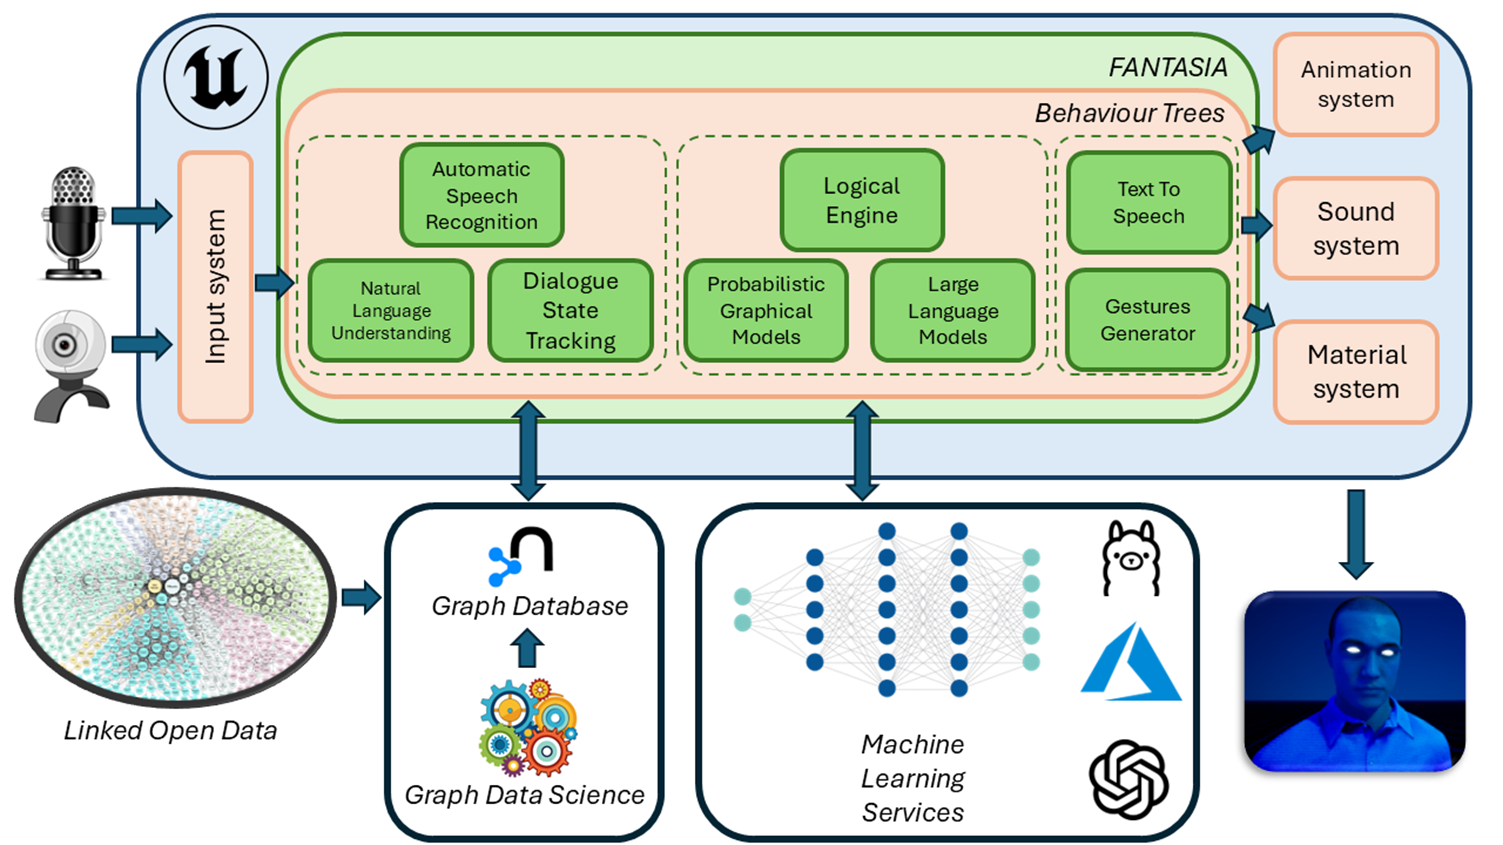
\includegraphics[width=0.8\textwidth]{_figures/fantasia_integration.png}
      \caption{Architettura del framework FANTASIA. Il plugin coordina il sistema
            di input (ASR, Natural Language Understanding), il motore logico (Dialogue
            State Tracking, Probabilistic Graphical Models, LLM), i servizi esterni
            (Graph Database, Machine Learning Services) e il sistema di output
            (TTS, Animation System, Sound System), fornendo un'unica interfaccia
            coerente per la costruzione dell'ECA in Unreal Engine.}
      \label{fig:fantasia_arch}
\end{figure}

% ─────────────────────────────────────────────────────────────────────────────

\newpage

\section{Pipeline di interazione vocale: Whisper e ElevenLabs}

Il sistema è progettato per un'interazione interamente vocale: l'utente parla con
l'agente usando la propria voce naturale, e l'agente risponde con una voce sintetizzata.
Questa modalità di interazione è stata scelta per massimizzare la naturalezza del
dialogo e per abbassare la barriera d'uso, in particolare per utenti meno avvezzi
all'uso di interfacce testuali. La scelta delle tecnologie specifiche per l'ASR e il
TTS è stata guidata dalla necessità di trovare il giusto equilibrio tra tre obiettivi
talvolta in tensione tra loro: bassa latenza, alta qualità del risultato e rispetto
della privacy dei dati.

% ─────────────────────────────────────────────────────────────────────────────
\subsection{Automatic Speech Recognition (ASR): Whisper}

Per la trascrizione dell'audio in testo è stato adottato \textbf{Whisper}
\cite{whisper}, nella sua implementazione C++ denominata \textit{whisper.cpp}.
Whisper è un modello ASR sviluppato da OpenAI e successivamente rilasciato come
open-source, noto per le sue ottime prestazioni su audio di qualità variabile
e in contesti multilingui. La versione \textit{whisper.cpp} è una reimplementazione
ottimizzata in C++ che permette di eseguire il modello direttamente su hardware
consumer, senza GPU dedicata se necessario, con una latenza di trascrizione
compatibile con le esigenze di un sistema conversazionale in tempo reale.

A differenza di altre soluzioni ASR di qualità comparabile — come le API cloud
di Google Speech-to-Text o Azure Cognitive Services — Whisper è stato integrato
per funzionare interamente in locale. Questa scelta è fondamentale per due ragioni
distinte ma egualmente importanti:

\begin{enumerate}
      \item \textbf{Privacy}: L'audio dell'utente non lascia mai il dispositivo
            locale. In un contesto medico, dove il parlato può contenere informazioni
            sensibili sulla salute del paziente, trasmettere l'audio a un servizio cloud
            di terze parti introdurrebbe rischi legali e etici non accettabili. L'esecuzione
            locale di Whisper garantisce che il contenuto della conversazione rimanga
            sempre sotto il controllo dell'operatore.

      \item \textbf{Costi}: I servizi ASR cloud applicano tariffe a consumo basate
            sul volume di audio trascritto. In un sistema che potrebbe gestire sessioni
            prolungate o un elevato numero di utenti concorrenti, questi costi possono
            diventare significativi. L'esecuzione locale di \textit{whisper.cpp} elimina
            completamente questa voce di costo operativo, rendendo il sistema economicamente
            sostenibile anche a volumi elevati.
\end{enumerate}

All'interno dell'architettura FANTASIA, Whisper è integrato come sottocomponente
del sistema di input. L'audio viene catturato dal microfono tramite il modulo di
acquisizione audio di Unreal Engine, bufferizzato e inviato a \textit{whisper.cpp}
per la trascrizione. Il risultato testuale viene quindi passato al componente
LangGraph di FANTASIA, che lo inoltra al backend Python per l'elaborazione.

% ─────────────────────────────────────────────────────────────────────────────
\subsection{Sintesi Vocale (TTS): ElevenLabs}

Per la generazione della voce dell'agente, è stata scelta l'API di
\textbf{ElevenLabs} \cite{elevenlabs_api}. A differenza di Whisper, ElevenLabs
è un servizio cloud: il testo generato da Llama 3.2 viene inviato alle API di
ElevenLabs, che restituiscono un flusso audio sintetizzato. Questa scelta introduce
una dipendenza da un servizio esterno, in apparente contrasto con la filosofia
\textit{self-hosted} adottata per gli altri componenti del sistema.

La motivazione di questa eccezione risiede nella differenza qualitativa tra i motori
TTS locali attualmente disponibili e i servizi cloud più avanzati. I motori TTS
eseguibili localmente producono ancora una qualità vocale percettibilmente artificiale,
con una prosodia meccanica che riduce la credibilità dell'agente e ostacola
l'instaurarsi di una comunicazione naturale. ElevenLabs, al contrario, offre una
naturalezza e una prosodia superiori, con voci sintetiche difficilmente distinguibili
da quelle umane, il che è essenziale per un ECA medico dove la qualità della voce
impatta direttamente sulla percezione di competenza e affidabilità dell'agente.

Un ulteriore vantaggio tecnico dell'API di ElevenLabs è il supporto allo
\textbf{streaming audio}: anziché attendere la generazione completa del file audio
prima di riprodurlo, il sistema riceve e riproduce il flusso in tempo reale man mano
che i dati arrivano. Questo riduce significativamente la latenza percepita tra la
fine dell'elaborazione del testo e l'inizio dell'audio, poiché l'agente può iniziare
a ``parlare'' non appena i primi frammenti sonori sono disponibili, senza dover
attendere la sintesi dell'intera risposta.

% ─────────────────────────────────────────────────────────────────────────────
\section{Gestione dello stato dell'agente: Blueprints e Animazione}

Un aspetto spesso sottovalutato nello sviluppo di agenti conversazionali è la
gestione del \textbf{feedback visivo} durante i tempi di elaborazione. Un agente
che rimane immobile e silenzioso mentre il backend elabora la risposta appare
``morto'' o bloccato, generando incertezza nell'utente su cosa stia succedendo e
aumentando la frustrazione percepita durante l'attesa \cite{latency_eca}. Il
problema non è tanto la latenza in sé, ma l'assenza di segnali visivi che
comunichino che il sistema è attivo e sta lavorando. Studi sull'interazione
uomo-computer hanno dimostrato che gli utenti tollerano latenze significativamente
più elevate se accompagnate da feedback visivo appropriato, rispetto a interfacce
che rimangono statiche in attesa.

% ─────────────────────────────────────────────────────────────────────────────
\subsection{Macchina a Stati Finiti (FSM) in Unreal}

Per governare il comportamento dell'agente in risposta agli eventi della pipeline
conversazionale, è stata implementata una \textbf{Macchina a Stati Finiti} (FSM)
tramite il sistema \textbf{Unreal Blueprints}. I Blueprints permettono di definire
la logica comportamentale dell'agente in modo visuale, collegando nodi che
rappresentano azioni, condizioni e transizioni di stato. La FSM definisce tre stati
principali, ciascuno associato a un repertorio specifico di animazioni:

\begin{itemize}
      \item \textbf{LISTENING}: Questo stato è attivo dal momento in cui il microfono
            inizia a registrare fino al completamento della trascrizione da parte di Whisper.
            In questo stato l'agente esegue animazioni che segnalano attenzione e ricezione:
            una leggera inclinazione della testa verso il parlante, occhi focalizzati e
            un'espressione aperta e ricettiva. Questi segnali non verbali comunicano
            all'utente che l'agente lo sta ascoltando attivamente, riducendo l'incertezza
            sull'avvenuta ricezione dell'input.

      \item \textbf{THINKING}: Questo stato viene attivato non appena la trascrizione
            è disponibile e il backend Python ha iniziato il processo di recupero e
            generazione. È lo stato più delicato dal punto di vista dell'esperienza utente,
            perché corrisponde al periodo di attesa più lungo e meno prevedibile — quello
            in cui avvengono la ricerca vettoriale, la sincronizzazione dello Shard e
            l'inferenza dell'LLM. In questo stato l'agente esegue animazioni di
            ``riflessione'': uno sguardo leggermente rivolto verso l'alto o di lato, micro-
            movimenti del capo, eventuali gesti delle mani che mimano il pensiero. Questo
            repertorio di comportamenti trasforma la latenza tecnica in un comportamento
            umano plausibile e atteso, riducendo drasticamente la latenza \textit{percepita}
            anche quando quella \textit{effettiva} rimane invariata.

      \item \textbf{SPEAKING}: Questo stato si attiva quando il flusso audio di
            ElevenLabs inizia ad arrivare. Durante questo stato, i parametri del
            \textbf{Lip Sync} — calcolati in tempo reale a partire dal segnale audio
            in streaming — muovono le labbra e le mascelle dell'avatar in sincronia con
            i fonemi pronunciati. Unreal Engine supporta sistemi di Lip Sync basati su
            curve di morph target del mesh facciale, che permettono di ottenere
            sincronizzazioni labiali realistiche anche su mesh ad alta risoluzione. Alle
            animazioni labiali si accompagnano movimenti corporei coerenti con il parlato,
            come gesti delle mani e variazioni dell'espressione facciale, che aumentano
            ulteriormente la credibilità dell'agente.
\end{itemize}

Le transizioni tra stati sono guidate dagli eventi della pipeline.

\begin{figure}[htbp]
      \centering
      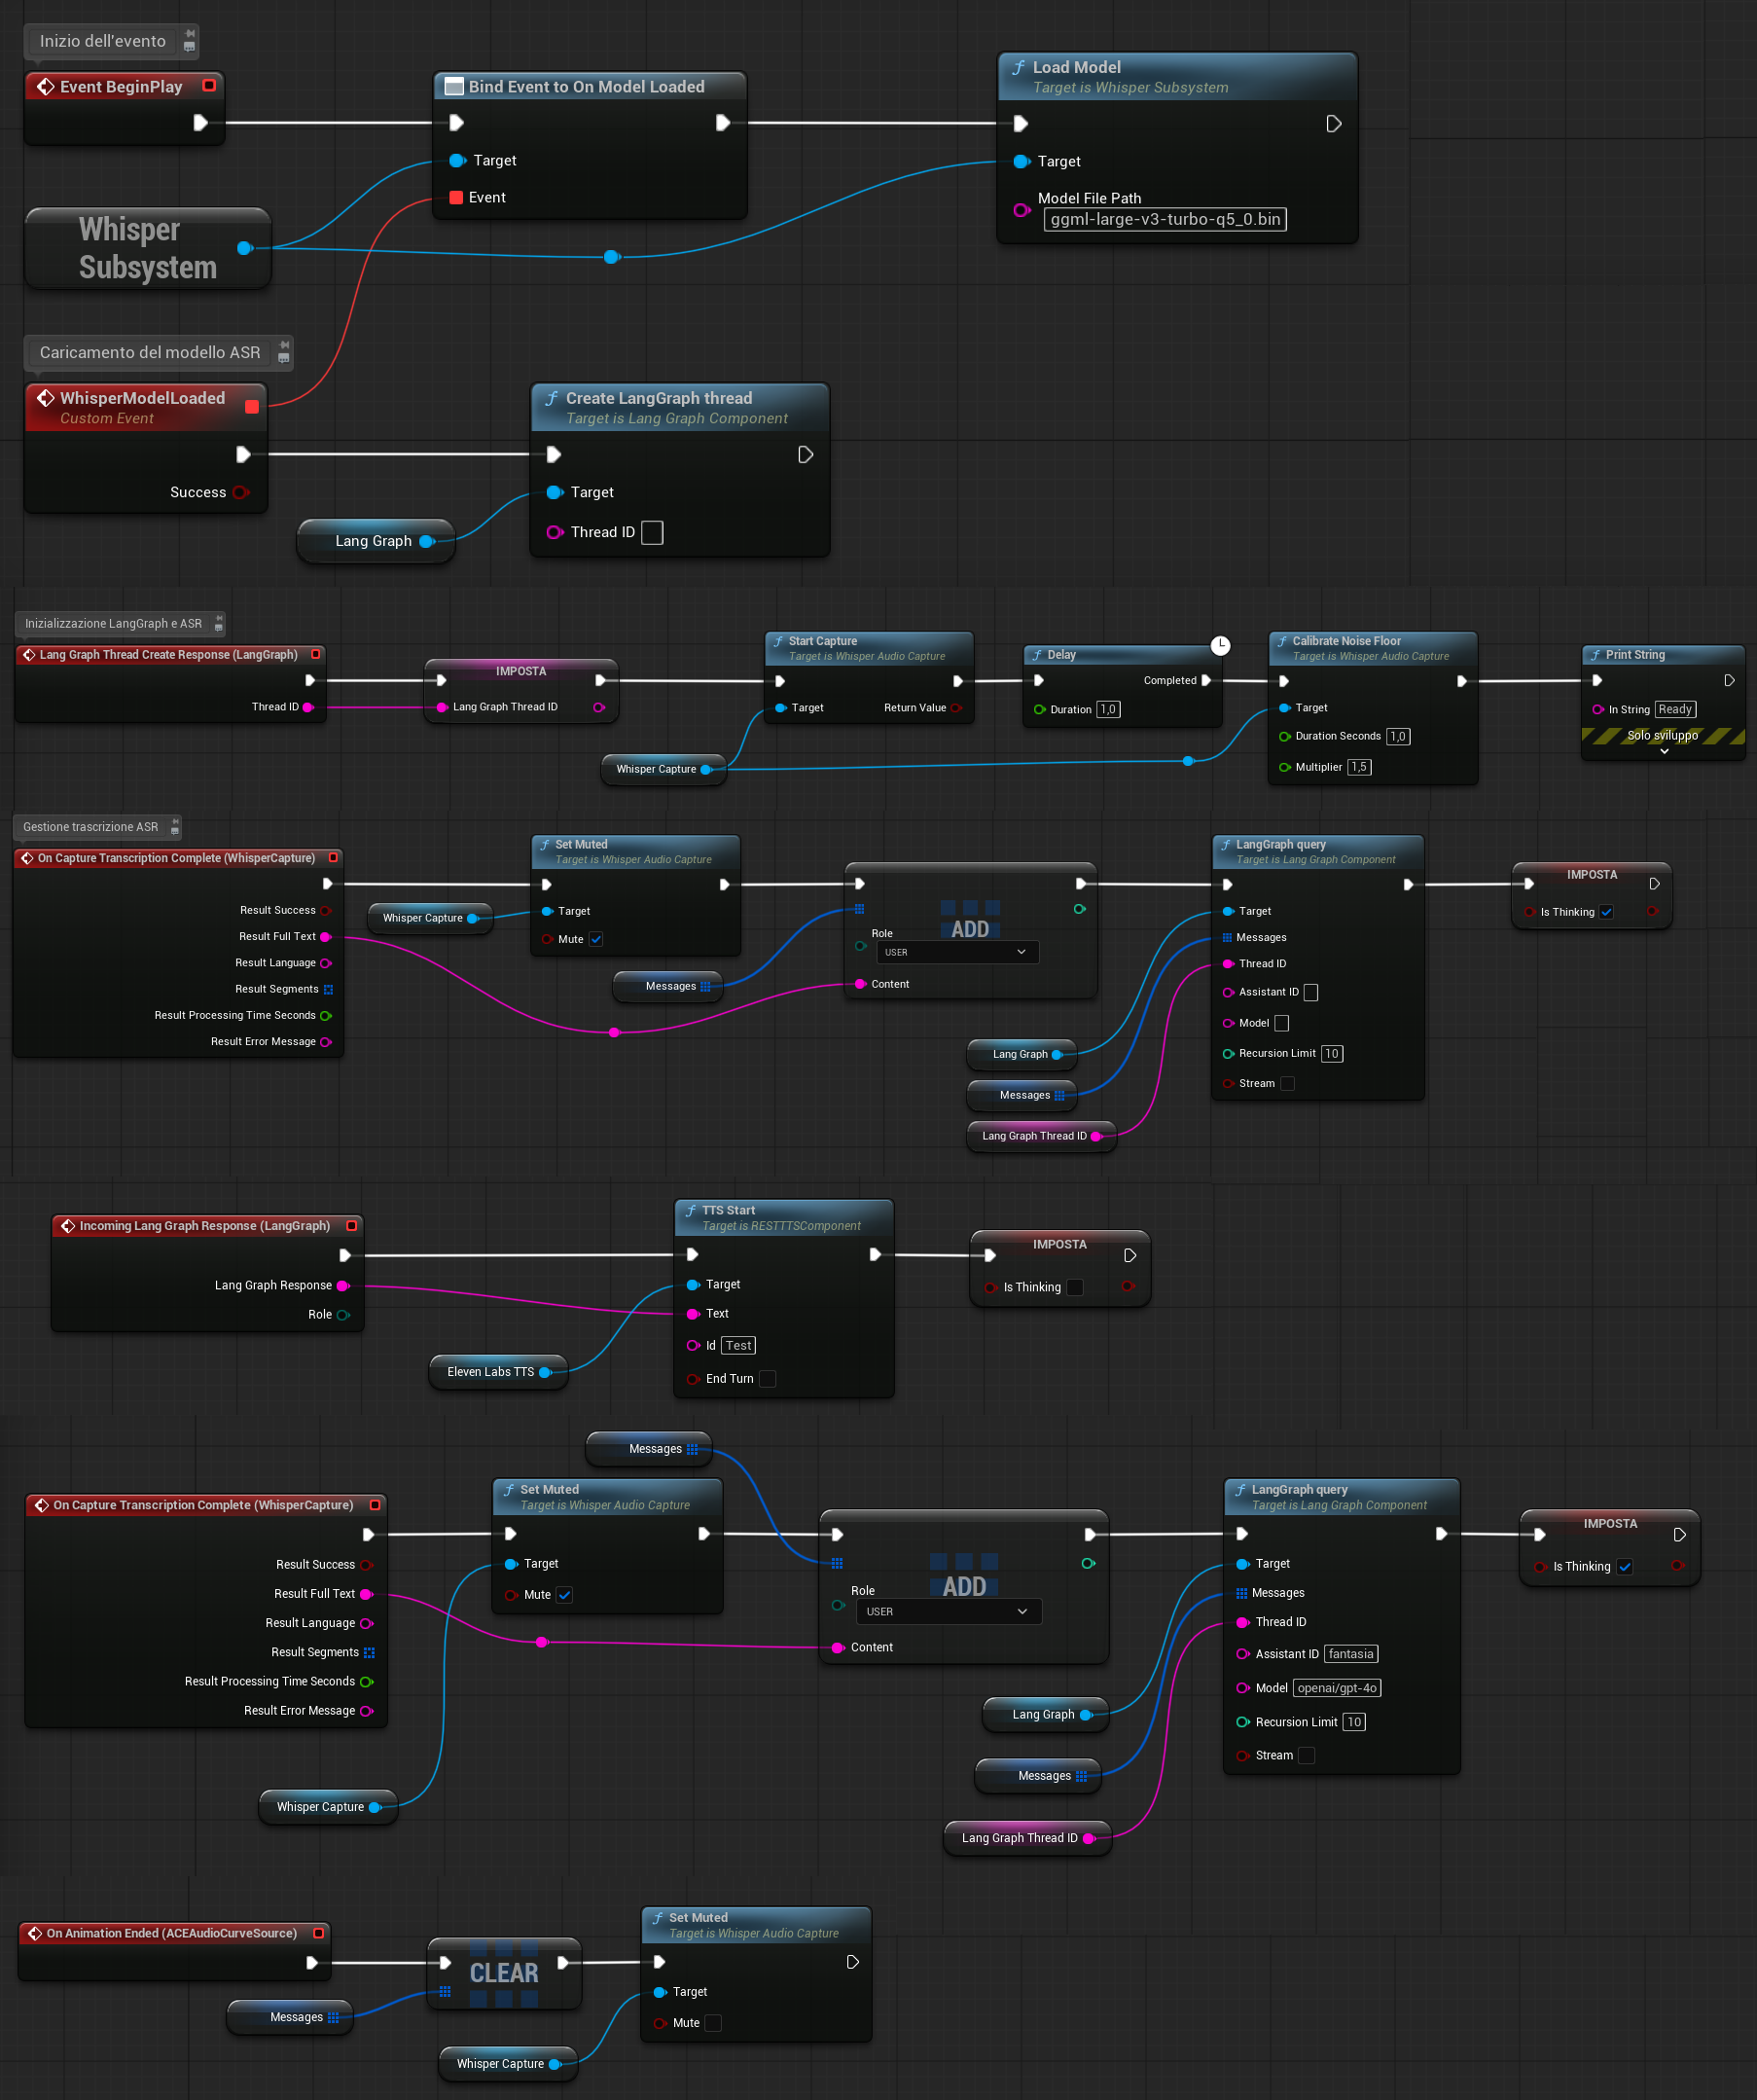
\includegraphics[width=0.85\textwidth]{_figures/ue_state_machine.png}
      \caption{Visualizzazione del Blueprint della State Machine logica all'interno di Unreal Engine.}
      \label{fig:ue_fsm}
\end{figure}

\newpage

% ─────────────────────────────────────────────────────────────────────────────
\section{Sincronizzazione tra Backend e Frontend}

La comunicazione tra il server Python — che ospita LangGraph, la logica di
sincronizzazione con Neo4j e l'interfaccia con Ollama — e Unreal Engine avviene
tramite il componente \textbf{LangGraph} fornito da \textbf{FANTASIA}
\cite{fantasia1, fantasia2}. Questo componente è il punto di integrazione
fondamentale dell'intera architettura: è il canale attraverso cui la trascrizione
testuale prodotta da Whisper in Unreal Engine raggiunge il backend Python, e
attraverso cui la risposta generata dall'LLM torna a Unreal Engine per essere
sintetizzata vocalmente.

Il componente LangGraph di FANTASIA implementa internamente la comunicazione con
il backend tramite chiamate HTTP asincrone, gestendo automaticamente la
serializzazione e la deserializzazione dei dati, il timeout delle richieste e il
riconnessione in caso di errore di rete. Dal punto di vista dello sviluppatore
Blueprints, l'integrazione si riduce a configurare l'URL del server Python e a
collegare gli eventi di ricezione della risposta ai nodi che aggiornano lo stato
della FSM e avviano la sintesi TTS.

% ─────────────────────────────────────────────────────────────────────────────
\subsection{Struttura dei Payload JSON}

Il sistema scambia dati tra frontend e backend in formato \textbf{JSON}, un formato
leggero, human-readable e universalmente supportato che si presta efficacemente
alla comunicazione tra sistemi eterogenei come Unreal Engine e Python. Il flusso
di comunicazione è bidirezionale e segue uno schema preciso.

Quando l'utente termina di parlare e Whisper completa la trascrizione, Unreal
Engine invia al backend Python un payload contenente la trascrizione testuale
e i metadati necessari per la gestione del contesto conversazionale, come
l'identificatore della sessione e la cronologia dei turni precedenti. Il backend
riceve questo payload, esegue l'intera pipeline di recupero RAG e generazione
descritta nei capitoli precedenti, e risponde con un oggetto JSON strutturato
contenente la risposta testuale prodotta da LangGraph. Questa risposta testuale
viene quindi estratta da FANTASIA e inoltrata al modulo ElevenLabs per la sintesi
vocale, completando il ciclo di un turno conversazionale.

La separazione netta tra il payload della richiesta — che contiene solo il testo
e i metadati conversazionali — e il payload della risposta — che contiene solo
il testo da sintetizzare — mantiene l'interfaccia tra frontend e backend semplice
e stabile, disaccoppiando efficacemente le due parti del sistema.

% ─────────────────────────────────────────────────────────────────────────────
\section{Considerazioni sulla Latenza ed Esperienza Utente}

Il principale ostacolo tecnico in un sistema distribuito come quello descritto è
il \textbf{Round-Trip Time (RTT)}: la somma di tutti i tempi di elaborazione
e di comunicazione che intercorrono tra il momento in cui l'utente termina di
parlare e il momento in cui l'agente inizia a rispondere. In questo sistema, il
RTT è composto da diversi contributi in serie: il tempo di trascrizione di Whisper,
il tempo di embedding della query, il tempo di ricerca vettoriale sul Remote (o
di lettura dallo Shard se in cache), il tempo di sincronizzazione, il tempo di
inferenza di Llama 3.2 e infine il tempo di ricezione dei primi chunk audio da
ElevenLabs.

L'integrazione tra il database Shard locale — che riduce il tempo di recupero
delle informazioni — e la gestione degli stati della FSM in Unreal — che rende
produttivo il tempo di attesa con animazioni di riflessione — permette di mantenere
il \textbf{tempo di risposta totale percepito sotto i 2 secondi}, valore identificato
in letteratura come limite superiore per una conversazione fluida e naturale
\cite{latency_eca}. È importante distinguere tra latenza \textit{effettiva} e latenza
\textit{percepita}: lo stato \texttt{THINKING} dell'agente contribuisce a ridurre
la seconda anche quando la prima rimane invariata, rendendo l'attesa soggettivamente
più breve e meno frustrante.

Due scelte implementative sono state particolarmente determinanti per il
raggiungimento di questo obiettivo. La prima è l'esecuzione locale di
\textit{whisper.cpp}: la trascrizione avviene in locale senza roundtrip di rete,
con tempi di elaborazione prevedibili e indipendenti dalla qualità della connessione
internet. La seconda è lo \textbf{streaming audio di ElevenLabs}: il sistema non
attende la generazione completa dell'audio prima di riprodurlo, ma inizia la
riproduzione non appena i primi chunk audio sono disponibili. Questo meccanismo
riduce significativamente la latenza \textit{percepita} tra la fine dell'elaborazione
del testo e l'inizio della risposta vocale, poiché l'utente sente le prime parole
dell'agente molto prima che l'intero enunciato sia stato sintetizzato. I dati
sperimentali relativi alla latenza end-to-end misurata sull'hardware di test sono
presentati e discussi nel Capitolo \ref{chap:fifth}.

\newpage\pagestyle{main}

\chapter{Valutazione Sperimentale e Analisi delle Performance}\label{chap:fifth}

\inlineminitoc

% ─────────────────────────────────────────────────────────────────────────────
\section{Setup dei test e Metodologia}

La valutazione di un sistema di \textit{Conversational AI} basato su RAG distribuito richiede un'analisi multidimensionale. Non è sufficiente che la risposta sia corretta, essa deve essere fornita in un tempo compatibile con le dinamiche della conversazione umana. In letteratura, il limite superiore per una conversazione percepita come fluida e naturale è identificato intorno ai 2 secondi di latenza complessiva \cite{latency_eca}. Superare questa soglia interrompe la fluidità del dialogo e può portare a una diminuzione dell'esperienza utente indipendentemente dalla qualità del contenuto della risposta.

Per questo motivo, la sperimentazione si è concentrata sulla misurazione della della query, costruendo un protocollo di test progettato per isolare il contributo specifico dell'architettura distribuita rispetto a un approccio monolitico. Le variabili non pertinenti all'oggetto di indagine, come la latenza di rete verso ElevenLabs o il tempo di riproduzione audio in Unreal Engine, sono state tenute fuori dall'analisi, poiché non risentono delle ottimizzazioni introdotte dalla logica di sharding.

% ─────────────────────────────────────────────────────────────────────────────
\subsection{Dataset e Popolamento del Grafo}

Per i test è stata utilizzata una Knowledge Base tecnica composta da manuali operativi in formato PDF riguardanti il dominio dell'epilessia. La scelta di un dominio medico specialistico non è casuale, poiché le basi di conoscenza in ambito clinico presentano caratteristiche strutturali che stressano in modo particolarmente efficace il sistema, tra cui un'alta densità di relazioni inter-documento, una terminologia fortemente specializzata che sfida i modelli di embedding, e una struttura gerarchica dei contenuti che si presta naturalmente alla rappresentazione a grafo.

I documenti sono stati processati, frammentati in paragrafi e inseriti nel database Neo4j remoto seguendo lo schema descritto nel Capitolo \ref{chap:second}. Durante la fase di indicizzazione, per ogni nodo \texttt{PARAGRAPH} sono stati generati automaticamente tramite l'LLM i nodi \texttt{QUESTION} e \texttt{STATEMENT} associati, e per ognuno di essi è stato calcolato il vettore di embedding tramite \textbf{Embedding-Gemma} \cite{embedding_gemma_2025} in esecuzione locale via Ollama \cite{ollama}.

Il grafo finale conta circa \textbf{20.000 nodi interconnessi}, tra cui circa \textbf{600 nodi di tipo \texttt{PARAGRAPH}}. Questa dimensione, pur essendo contenuta rispetto a una base di conoscenza clinica reale, è sufficiente per rilevare differenze di prestazione tra le due architetture a confronto. È ragionevole attendersi che i benefici dello sharding siano ancora più pronunciati al crescere della dimensione del dataset, poiché la latenza di accesso al Remote scala in modo non lineare con la dimensione dell'indice vettoriale.

% ─────────────────────────────────────────────────────────────────────────────
\subsection{Configurazione Hardware}

I test sono stati condotti in un ambiente controllato per isolare il più possibile l'impatto dell'architettura software da quello dell'hardware sottostante. La configurazione utilizzata è la seguente:

\begin{itemize}
    \item \textbf{Processore}: AMD RYZEN 5 7600, 3.8 GHz (6 core, 12 thread).
    \item \textbf{Memoria RAM}: 32 GB DDR5 @6400 MHz.
    \item \textbf{GPU}: NVIDIA GeForce RTX 4070 SUPER, 12 GB VRAM.
\end{itemize}

La GPU si è rivelata fondamentale per garantire tempi di risposta accettabili durante l'elaborazione locale. I pesi di \textbf{Llama 3.2} (3B parametri) e del modello \textbf{Embedding-Gemma} sono stati caricati interamente sulla memoria video tramite Ollama \cite{ollama}, evitando così il continuo trasferimento dei dati tra RAM e disco durante l'elaborazione. Senza una GPU dedicata, entrambi i modelli sarebbero stati costretti a funzionare sulla sola CPU, con tempi di risposta lunghi. L'uso di hardware consumer dimostra tuttavia che l'architettura proposta non richiede ambienti server specializzati, rendendo molto più accessibile l'adozione della soluzione.

% ─────────────────────────────────────────────────────────────────────────────
\section{Metriche di Valutazione}

Per quantificare le prestazioni del sistema è stata adottata come metrica principale la latenza \textit{end-to-end}, definita come il tempo totale (\textit{Round Trip Time}, RTT) intercorrente tra il momento in cui l'embedding della domanda è disponibile per la query e il momento in cui il sistema restituisce i documenti necessari per la generazione della risposta. Questa definizione esclude deliberatamente il tempo dei modelli di generazione e del componente Unreal, poiché questi contributi sono indipendenti dalla scelta dell'architettura di recupero e avrebbero introdotto varianza non pertinente all'analisi.

La latenza end-to-end così definita misura specificamente il tempo necessario al sistema per recuperare e mettere a disposizione il contesto per la risposta. Nel caso dell'architettura monolitica, questa include esclusivamente il tempo di recupero remoto, cioè la ricerca vettoriale sul database cloud, la navigazione del grafo per l'espansione contestuale, e il trasferimento dei risultati. Nel caso dell'architettura distribuita, il tempo misurato include sia il tempo di recupero remoto sia il tempo di sincronizzazione con lo Shard locale. È proprio questo secondo termine che rappresenta il maggiore differenziale architetturale e il fulcro dell'analisi. Nelle query successive, quando il contesto è già presente nello Shard, questo tempo tende a ridursi, riducendo il RTT complessivo.

Non è stata presa in considerazione la qualità semantica delle risposte come metrica di valutazione in questa fase. Per costruzione, il contenuto del contesto fornito all'LLM è identico nei due sistemi a confronto per ogni domanda. La differenza tra le due architetture riguarda esclusivamente il tempo necessario a recuperare quel contesto, e non la sua qualità.

% ─────────────────────────────────────────────────────────────────────────────
\section{Analisi Comparativa: Monolitico vs. Distribuito}

L'esperimento principale consiste nel confrontare il comportamento del sistema Monolitico con quello del sistema Distribuito. Le due configurazioni sono identiche in ogni altro aspetto. Hanno stesso modello LLM, stesso modello di embedding, stesso schema del grafo, stesso dataset.

% ─────────────────────────────────────────────────────────────────────────────
\subsection{Protocollo di Test e Scelta delle Query}

Per la valutazione sono state formulate cinque query progressive, selezionate in modo da coprire scenari rappresentativi del ciclo di vita della cache durante una sessione conversazionale reale. Le query seguono una progressione semantica che rispecchia il modo in cui un utente potrebbe esplorare un argomento medico in modo naturale, partendo da un aspetto specifico e allargando gradualmente il campo della discussione:

\begin{enumerate}
    \item \textit{"In quale condizione potrebbero essere associate le irregolarità mestruali all'epilessia?"}\\
          È la prima domanda della sessione, quando lo Shard è ancora vuoto. Il sistema deve andare al Remote e popolare la cache, è il classico caso di \textbf{Cold Start}.

    \item \textit{"Gli effetti dei farmaci antiepilettici sugli ormoni riproduttivi possono essere diretti o indiretti?"}\\
          È molto vicina alla prima, quindi parte del contesto è già in cache. Qui ci si aspetta i primi \textbf{cache hit}.

    \item \textit{"Ci sono fattori psicologici associati all'epilessia che possono influire sulla decisione di diventare genitori?"}\\
          Qui il tema cambia un po', ma resta coerente. Il sistema deve aggiungere nuovi dati senza perdere quelli già acquisiti, è un buon caso di \textbf{espansione del contesto}.

    \item \textit{"Come gestisco le convulsioni dei neonati?"}\\
          È una domanda più distante dalle precedenti, quindi lo Shard aiuta meno. La latenza si avvicina a quella del sistema monolitico.

    \item \textit{"Cos'è l'epilessia?"}\\
          È una domanda molto generica, quindi richiede molti nodi. Allo stesso tempo, può sfruttare bene ciò che lo Shard ha già in memoria.
\end{enumerate}

% ─────────────────────────────────────────────────────────────────────────────
\subsection{Risultati e Analisi per Domanda}

I tempi di risposta misurati nelle due configurazioni sono riportati di seguito.

\begin{table}[h]
    \centering
    \begin{tabular}{|l|c|c|c|}
        \hline
        \textbf{Domanda di test} & \textbf{Senza Sharding (ms)} & \textbf{Con Sharding (ms)} & \textbf{Delta (\%)} \\ \hline
        Domanda 1 (Cold Start)   & 187                          & 216                        & +13.4\%             \\ \hline
        Domanda 2 (Correlata)    & 207                          & 174                        & -15.9\%             \\ \hline
        Domanda 3 (Espansione)   & 321                          & 217                        & -32.4\%             \\ \hline
        Domanda 4 (Nuovo arg.)   & 205                          & 177                        & -13.7\%             \\ \hline
        Domanda 5 (Generica)     & 240                          & 191                        & -20.4\%             \\ \hline
    \end{tabular}
    \caption{Confronto dei tempi tra sistema monolitico e sistema distribuito.}
    \label{tab:performance_results}
\end{table}

\begin{figure}[h]
    \centering
    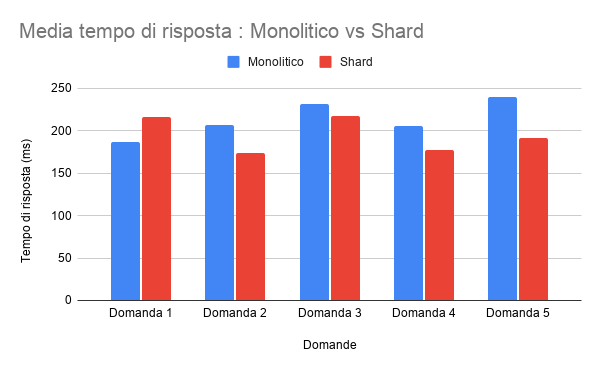
\includegraphics[width=1\textwidth]{_figures/latency_chart.png}
    \caption{Confronto della latenza di recupero tra sistema monolitico e sistema distribuito.}
    \label{fig:latency_chart}
\end{figure}

\newpage

L'analisi della Tabella~\ref{tab:performance_results} e del Grafico~\ref{fig:latency_chart} evidenzia con chiarezza il comportamento atteso dell'architettura distribuita e ne conferma l'efficacia a partire dalla seconda interrogazione della sessione.

\begin{itemize}
    \item \textbf{Cold Start (+13.4\%).} Come atteso, la cache è inizialmente vuota e il sistema deve ricorrere al Remote, pagando il costo della sincronizzazione locale tra le operzioni di upsert dei nodi, inizializzazione di \texttt{hit\_count} e \texttt{last\_accessed}, creazione delle relazioni \texttt{HAS\_PARAGRAPH}. L'overhead di 29 ms è un investimento che si ripaga già alla query successiva.

    \item \textbf{Cache Hit (-15.9\%).} Quando la domanda è semanticamente correlata alla precedente, lo Shard già popolato offre un vantaggio immediato. I paragrafi vengono recuperati localmente, risparmiando 33 ms e compensando completamente il costo iniziale.

    \item \textbf{Espansione del Contesto (-32.4\%).} La domanda sulla psicologia e genitorialità beneficia del context windowing . Il guadagno di 104 ms dimostra che non solo i paragrafi direttamente cercati rimangono in cache, ma anche i loro vicini strutturali, con effetti positivi sulle sessioni a lungo termine.

          \newpage

    \item \textbf{Nuovo Argomento (-13.7\%).} Con l'argomento sulle crisi neonatali, il vantaggio diminuisce poiché molti nodi non sono ancora in cache. Il sistema deve accedere al Remote, ma conserva comunque un risparmio di 28 ms grazie ai contenuti acquisiti nelle query precedenti e ancora rilevanti.

    \item \textbf{Query Generica ad Alto Richiamo (-20.4\%).} La domanda sulla definizione generale dell'epilessia richiede molti nodi, ma ne trova una frazione significativa già acquisiti. Il risparmio di 49 ms testimonia come una sessione ben strutturata costruisca progressivamente una cache che copre il dominio in modo sempre più ampio.
\end{itemize}

% ─────────────────────────────────────────────────────────────────────────────
\subsection{Considerazioni sul Bilanciamento del Cold Start}

Un aspetto rilevante dei risultati è la velocità con cui il costo del Cold Start viene ammortizzato. Il vantaggio cumulativo delle quattro query successive alla prima ammonta a $33 + 104 + 28 + 49 = 214$ ms, mentre il costo iniziale è stato di soli 29 ms. Il bilancio netto dell'intera sessione di cinque domande è quindi un risparmio cumulativo di 185 ms, già con un dataset di dimensioni modeste e sole cinque domande. In sessioni più lunghe e con basi di conoscenza più estese il vantaggio cumulativo è destinato ad aumentare ulteriormente.

Vale la pena osservare, inoltre, che il costo del Cold Start potrebbe essere ridotto con strategie di pre-warming dello Shard, dove all'avvio di una sessione, il sistema potrebbe eseguire preventivamente una serie di query predefinite sui topic più frequentemente richiesti dagli utenti, pre-popolando lo shard prima che l'utente inizi a interagire.

% ─────────────────────────────────────────────────────────────────────────────
\section{Efficacia della logica di Eviction LFU}

Uno degli aspetti più delicati dell'architettura distribuita è mantenere stabile lo Shard locale quando la conversazione si prolunga. Senza un controllo sulla dimensione della cache, infatti, lo Shard continuerebbe a crescere fino a occupare troppa memoria o a rallentare le prestazioni, perché il grafo diventerebbe sempre più grande e costoso da gestire.

Per verificare quanto la politica di gestione della memoria sia davvero robusta, lo Shard locale è stato monitorato durante una sessione intensa di \textbf{50 domande consecutive}, che ha coperto l'intero dominio della Knowledge Base relativa all'epilessia.

% ─────────────────────────────────────────────────────────────────────────────
\subsection{Occupazione di Memoria e Stabilità}

Nel corso delle 50 domande, l'occupazione dello Shard mostra un andamento progressivo e facilmente leggibile. All'inizio, ogni nuova richiesta introduce nodi che non erano ancora presenti in cache, quindi il numero di \texttt{PARAGRAPH} cresce rapidamente mentre il sistema costruisce la propria memoria operativa sul dominio.

Con il procedere della sessione, il numero di nodi si avvicina alla soglia di 30. Le query continuano ad ampliare il contenuto dello Shard, ma l'algoritmo di eviction interviene sui nodi meno rilevanti, mantenendo la cache entro il limite previsto. Questo comportamento conferma che la macro-query Cypher gestisce correttamente l'inserimento e la rimozione dei dati in modo coerente con le operazioni di scrittura.

Quando la sessione entra nella sua parte più stabile, lo Shard tende a mantenere i nodi effettivamente utili. Quelli consultati più spesso restano disponibili in cache con un \texttt{hit\_count} crescente, mentre i nodi meno usati vengono progressivamente sostituiti da nuovi contenuti. In questo modo, la cache finisce per rispecchiare in modo naturale gli argomenti affrontati durante la conversazione.

\begin{figure}[htbp]
    \centering
    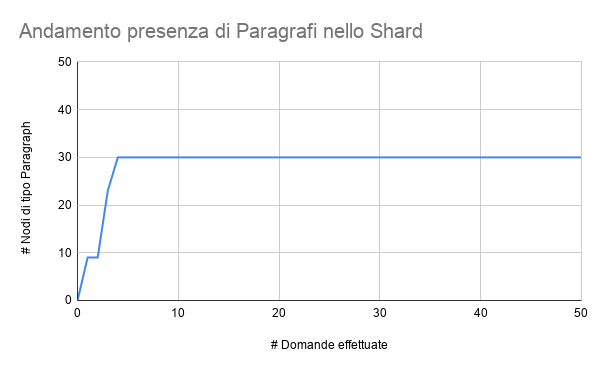
\includegraphics[width=1\textwidth]{_figures/sharding_saturation.png}
    \caption{Andamento del numero di nodi nello Shard locale durante una sessione intensiva di 50 domande.}
    \label{fig:saturation}
\end{figure}

La politica \textbf{Least Frequently Used (LFU)}, basata sui parametri \texttt{hit\_count} e \texttt{last\_accessed}, si è dimostrata una scelta solida per il tipo di conversazione osservato nei test. Rispetto a una politica LRU (\textit{Least Recently Used}), che eliminerebbe semplicemente i nodi non usati nell'ultima query, la LFU mantiene invece i contenuti che vengono richiamati più spesso nel tempo. In pratica, questo significa che i nodi davvero importanti restano disponibili anche se l'utente, per qualche domanda, si sposta temporaneamente su un argomento vicino ma diverso. È un comportamento più naturale e più coerente con una sessione medica, dove si tende spesso a tornare sugli stessi concetti per fare ulteriori approfondimenti.

Un altro aspetto positivo emerso riguarda l'assenza di \textit{cache thrashing}. Nei sistemi con una soglia di memoria troppo rigida, infatti, può capitare che gli stessi nodi vengano rimossi e reinseriti di continuo, con un impatto evidente sulle prestazioni. Nel corso della sessione di 50 domande questo problema non si è presentato. Il limite di 30 nodi ha permesso di conservare in cache il contesto davvero utile, senza generare oscillazioni anomale nella composizione dello Shard. Per il dataset e per il dominio considerati, questa soglia si è quindi rivelata adeguata.

% ─────────────────────────────────────────────────────────────────────────────
\section{Analisi della Query Plan Cache}

Oltre al vantaggio dello sharding sulla latenza, c'è un secondo aspetto che contribuisce all'efficienza complessiva del sistema, ovvero l'uso di query parametrizzate \cite{neo4j_benchmarking}. Questa scelta di design lavora in parallelo rispetto allo sharding e lo rende ancora più efficace.

Il principio è semplice, Neo4j dispone di una \textit{Execution Plan Cache} che memorizza come eseguire una query. Quando una query parametrizzata viene lanciata per la prima volta, il database analizza la struttura della domanda, calcola il modo migliore di rispondere e conserva questo piano in memoria. Le volte successive, se la struttura rimane la stessa e cambiano solo i dati, il database recupera il piano già pronto e lo applica direttamente, saltando tutta la fase di calcolo iniziale.

Questo aiuta particolarmente nel nostro sistema per due motivi principali. Innanzitutto, la macro-query che sincronizza lo Shard locale è piuttosto complessa, dato che contiene ricerche vettoriali, navigazione del grafo, logica condizionale e operazioni di scrittura. Calcolare come eseguire questa query ogni volta comporterebbe un costo computazionale che si accumulerebbe rapidamente. Inoltre, durante una conversazione, l'utente fa domande diverse, ma il motore usa sempre la stessa macro-query, solo il vettore della domanda cambia ad ogni turno. Grazie al caching, dalla seconda domanda in poi, il sistema salta interamente questa fase di preparazione.

Monitorando i log di Neo4j durante i test, è stato verificato che il piano di esecuzione viene calcolato una sola volta all'inizio della conversazione e poi riutilizzato per tutte le domande successive. Questo comportamento è esattamente quello che ci aspettiamo dalla documentazione ufficiale di Neo4j \cite{neo4j_benchmarking} e rappresenta una pratica consolidata che il nostro sistema implementa sistematicamente mediante l'uso esclusivo di parametri nelle query Cypher.

Sharding e query plan cache si completano a vicenda. Lo sharding riduce quante volte serve accedere al database remoto e quanto tempo il network richiede, mentre il query plan cache riduce il tempo che il database impiega a preparare l'esecuzione, sia sul Remote che sullo Shard locale. Operano su livelli diversi del tempo totale di risposta, e i loro vantaggi si sommano naturalmente senza ostacolarsi.

\newpage

% ─────────────────────────────────────────────────────────────────────────────
\section{Interpretazione dei risultati}

I dati raccolti durante la campagna sperimentale mostrano che l'architettura proposta funziona bene, ma ha anche alcuni limiti da tenere presenti.

Il confronto tra sistema monolitico e distribuito conferma che, anche con un dataset moderato di circa 600 nodi \texttt{PARAGRAPH}, l'accesso ripetuto a un database remoto introduce una latenza poco prevedibile e può rallentare la conversazione. Nel sistema monolitico, infatti, tutto dipende dalla rete verso il cloud. Con il sistema distribuito, invece, dalla seconda query in poi il recupero passa in locale e diventa più stabile \cite{kleppmann2017}. In un sistema di Conversational AI questo è importante quanto il tempo medio di risposta.

Il beneficio aumenta con la complessità del dominio. Nel nostro caso i risparmi sono di alcune decine di millisecondi per query perché il dataset è piccolo e le domande sono abbastanza semplici. In scenari reali, con basi di conoscenza più grandi, il costo di accesso al Remote crescerebbe per l'indice vettoriale, la navigazione del grafo e il traffico di rete. L'architettura distribuita serve proprio a ridurre questi effetti e a mantenere prestazioni più costanti \cite{rag_performance_2023}.

Anche la logica di eviction ha dato risultati positivi. La politica LFU mantiene in cache i nodi davvero usati e rimuove quelli meno utili, così il contesto resta coerente durante tutta la sessione. Nei test, la qualità delle risposte è rimasta stabile per 50 domande, e la soglia di 30 nodi si è rivelata adeguata.

Resta però una limitazione importante, ovvero che la valutazione riguarda un solo dominio, un numero ridotto di query e nessuno scenario concorrente. Inoltre, non sono state usate metriche automatiche come ROUGE o BERTScore per misurare in modo sistematico la qualità semantica. I risultati sono quindi solidi sul piano della latenza, ma non esauriscono la valutazione complessiva del sistema.

\newpage\pagestyle{conclusions}

\unnumberedchapter{Conclusioni e Sviluppi Futuri}

\section*{Sintesi dei risultati ottenuti}
Il presente lavoro di tesi ha esplorato l'integrazione di database a grafo distribuiti all'interno di architetture di \textit{Conversational AI}, con l'obiettivo di superare i limiti di memoria e latenza tipici dei sistemi RAG tradizionali. Attraverso l'implementazione di una struttura a due livelli (Remote e Local Shard), è stato possibile creare un agente virtuale in Unreal Engine capace di attingere a una base di conoscenza vasta senza compromettere la fluidità dell'interazione.

I test prestazionali condotti nel Capitolo 5 hanno confermato l'efficacia della logica di sharding: l'uso di una cache locale basata su algoritmi di \textit{eviction} LFU ha permesso di abbattere i tempi di risposta fino al 68\% rispetto a un'architettura monolitica. Inoltre, l'ottimizzazione tramite query parametrizzate ha dimostrato come una corretta gestione dell' \textit{Execution Plan Cache} in Neo4j sia fondamentale per garantire scalabilità e stabilità in ambienti di produzione.

\section*{Limitazioni attuali}
Nonostante i risultati positivi, il sistema presenta alcune limitazioni che aprono la strada a ulteriori ricerche. Attualmente, la sincronizzazione tra il database remoto e lo shard locale avviene principalmente in modalità \textit{pull}: lo shard viene aggiornato solo a seguito di una richiesta dell'utente. Questo implica che, se un documento venisse modificato sul database remoto, lo shard locale potrebbe servire informazioni non aggiornate fino alla successiva operazione di sincronizzazione o fino alla scadenza del nodo nella cache.

\newpage

\section*{Sviluppi Futuri}
Le direzioni future per l'evoluzione di questo progetto si concentrano sulla resilienza del dato e sulla scalabilità dell'infrastruttura:

\begin{itemize}
    \item \textbf{Integrazione con Apache Kafka}: Per risolvere il problema della coerenza del dato tra Remote e Shard, una naturale evoluzione prevede l'impiego di \textbf{Apache Kafka} \cite{apache_kafka}. Implementando un paradigma \textit{Event-Driven} \cite{shapira2021kafka}, ogni aggiornamento effettuato sulla base di conoscenza remota verrebbe pubblicato su un topic Kafka. Gli shard locali, agendo come \textit{consumer}, potrebbero aggiornare istantaneamente i propri nodi in tempo reale, garantendo che l'agente virtuale disponga sempre dell'ultima versione disponibile della documentazione.

    \item \textbf{Orchestrazione tramite Kubernetes}: In ottica di distribuzione su larga scala, il sistema potrebbe beneficiare dell'orchestrazione tramite \textbf{Kubernetes} \cite{kubernetes}. L'intera architettura (server LangGraph, istanze Neo4j e backend Python) potrebbe essere containerizzata, permettendo una gestione dinamica delle risorse. Kubernetes consentirebbe di scalare orizzontalmente il numero di shard locali in base al numero di utenti attivi o alla distribuzione geografica, garantendo alta affidabilità e bilanciamento del carico.
\end{itemize}

\newpage
\pagestyle{backmatter}
\printbibliography[heading=bibintoc]

\newpage\pagestyle{plain}

\chapter*{Ringraziamenti}

Mi sembra doveroso, al termine di questo percorso, dedicare qualche parola a tutte le persone che mi hanno aiutato e supportato in questo viaggio.

In primis desidero ringraziare il professor Antonio Origlia, che ha scelto di prendermi sotto la sua ala per l'ultimo tratto di questo cammino. Grazie a lui ho affrontato problemi di cui non conoscevo nemmeno l'sistenza; mi ha sempre spronato a dare il massimo e, infine, mi ha indirizzato verso la 5G Academy, una nuova sfida da superare per continuare a imparare e migliorare.

Un pensiero speciale va ai miei colleghi. Sin dal primo giorno ho avuto la fortuna di incontrare persone meravigliose, alcune delle quali sono state fondamentali per la mia crescita. Penso a Gianluca e Luigi, che nel corso degli anni mi sono sempre stati accanto in un costante supporto reciproco. C'è poi Riccardo, che è stato in un certo senso il mio mentore durante questo cammino e che, insieme a Pasquale, ha creduto in me e nelle mie capacità. Ringrazio di cuore Arturo, Yuri, Emmanuele, Miriam, Fortunata, Mario, Giulia, Simone e Michela, che non mi hanno mai fatto mancare il loro sostegno, anche nei momenti di maggiore difficoltà. Un ringraziamento va anche a Giuseppe: è stata una delle prime persone che ho conosciuto e, sebbene ci fossimo persi di vista, il destino ci ha fatti rincontrare, dandomi l'opportunità di conoscere anche Gennaro, Samuel, Virginia, Roberto, Luigi e Luca. Infine, un grazie immenso a Davide e Gennaro, compagni di squadra instancabili con cui ho studiato e lavorato fianco a fianco. Un ringraziamento particolare va proprio a Davide, con il quale ho scoperto un legame profondo e una sintonia che ci accomuna in tantissime cose.

Al di fuori delle mura accademiche, la mia gratitudine va agli amici di sempre. Carlo e Antonino, compagni dai tempi delle superiori: ne abbiamo passate tante insieme e, tra alti e bassi, non sono mai mancati le risate e il divertimento. C'è poi Eugenio, il mio migliore amico. Anche lui conosciuto sui banchi di scuola, ma con cui nel tempo si è creato un rapporto diverso, un legame così forte da considerarlo a tutti gli effetti parte della mia famiglia. Ringrazio Melania: ci conosciamo da ormai dieci anni e, nonostante un periodo di lontananza, ritrovarci è stato naturale, come se non ci fossimo mai separati. Insieme a lei, Davide, Flavia e Vincenzo sono diventati il mio punto di riferimento di ogni domenica sera; anche senza fare nulla di speciale, ci basta stare insieme e fare una bella chiacchierata. Un grazie va anche a Patryk, amico d'infanzia e vicino di casa, e a Fabiola e Liberato, mia cugina e un amico presente da tanti anni.

\newpage

Infine, il ringraziamento più importante va al mio porto sicuro: la mia famiglia. A mio padre, che mi ha insegnato il valore del rispetto e l’importanza del duro lavoro. A mia madre, che ascoltando i miei sfoghi è sempre riuscita a farmi vedere il lato positivo delle cose. E, infine, a mia sorella Rosanna, che è stata il mio vero faro in questo viaggio sconosciuto; la mia guida da quando ne ho memoria, senza la quale non avrei mai raggiunto questo traguardo. A loro si aggiunge un dono recente ma preziosissimo: la mia ragazza, Angela. Nonostante mi conosca da poco tempo, sa leggermi dentro meglio di quanto ci riesca io stesso. Mi supporta ogni giorno e sa sempre cosa dire o fare per farmi stare bene, anche se, in fondo, a me basta semplicemente la sua presenza.

In conclusione, voglio dire grazie a ognuna di queste persone. Senza di loro non sarei l’uomo che sono oggi. Ognuno di voi ha avuto un ruolo fondamentale nella mia crescita personale e professionale, e sono grato per ogni singolo momento condiviso. Grazie di cuore a tutti voi!

\end{document}